
\chapter{Josué}

\section*{Introducción al Libro de Josué}

El \textbf{Libro de Josué} es el primero de los llamados \textbf{Libros Históricos} en el Antiguo Testamento, y su nombre se debe a su protagonista principal, \textbf{Josué}, quien fue el sucesor de Moisés como líder del pueblo de Israel. Este libro narra la conquista y ocupación de la \textbf{Tierra Prometida}, Canaán, bajo la dirección de Josué, cumpliendo así las promesas hechas por Dios a Abraham, Isaac y Jacob.

\subsection*{Autoría}

La tradición judía y cristiana atribuyen la redacción del libro de Josué a \textbf{Josué mismo}, especialmente las secciones que relatan su liderazgo y conquistas. Sin embargo, estudios modernos sugieren que el libro fue compilado posteriormente, posiblemente durante el período del exilio babilónico (siglo VI a.C.) o poco después, como parte de la tradición deuteronomista. Este enfoque resalta la importancia de la obediencia a la ley de Dios como clave para el éxito y la prosperidad de Israel.

\subsection*{Temática}

El libro de Josué se centra en la conquista de la Tierra Prometida y la distribución de sus territorios entre las tribus de Israel. Sus temas principales incluyen:
\begin{itemize}
	\item \textbf{La conquista de Canaán} (Josué 1–12): Relata la entrada de Israel en la Tierra Prometida, comenzando con el cruce del río Jordán y la caída de Jericó, hasta las principales campañas militares dirigidas por Josué.
	\item \textbf{Distribución de la Tierra} (Josué 13–22): Narra cómo las tierras conquistadas se dividen entre las doce tribus de Israel, subrayando el cumplimiento de las promesas divinas.
	\item \textbf{Fidelidad al pacto} (Josué 23–24): Josué, al final de su vida, exhorta al pueblo a permanecer fiel al pacto con Dios y a evitar la idolatría, reafirmando la alianza en Siquem.
\end{itemize}



El libro de Josué está profundamente enraizado en las tradiciones históricas y teológicas de Israel. Aunque los relatos de la conquista de Canaán pueden reflejar un proceso más gradual según la evidencia arqueológica, el libro subraya la intervención divina como el elemento central en el establecimiento de Israel en la Tierra Prometida. Este énfasis refleja la intención de mostrar cómo el cumplimiento de las promesas de Dios está ligado a la obediencia y la fidelidad del pueblo.


El libro de Josué no solo relata eventos históricos, sino que también sirve como un recordatorio teológico de la fidelidad de Dios y de las responsabilidades del pueblo de Israel bajo el pacto. A través de la figura de Josué, se muestra el modelo de un líder obediente y fiel, que confía plenamente en la guía divina para cumplir la misión encomendada.



\begin{center}
	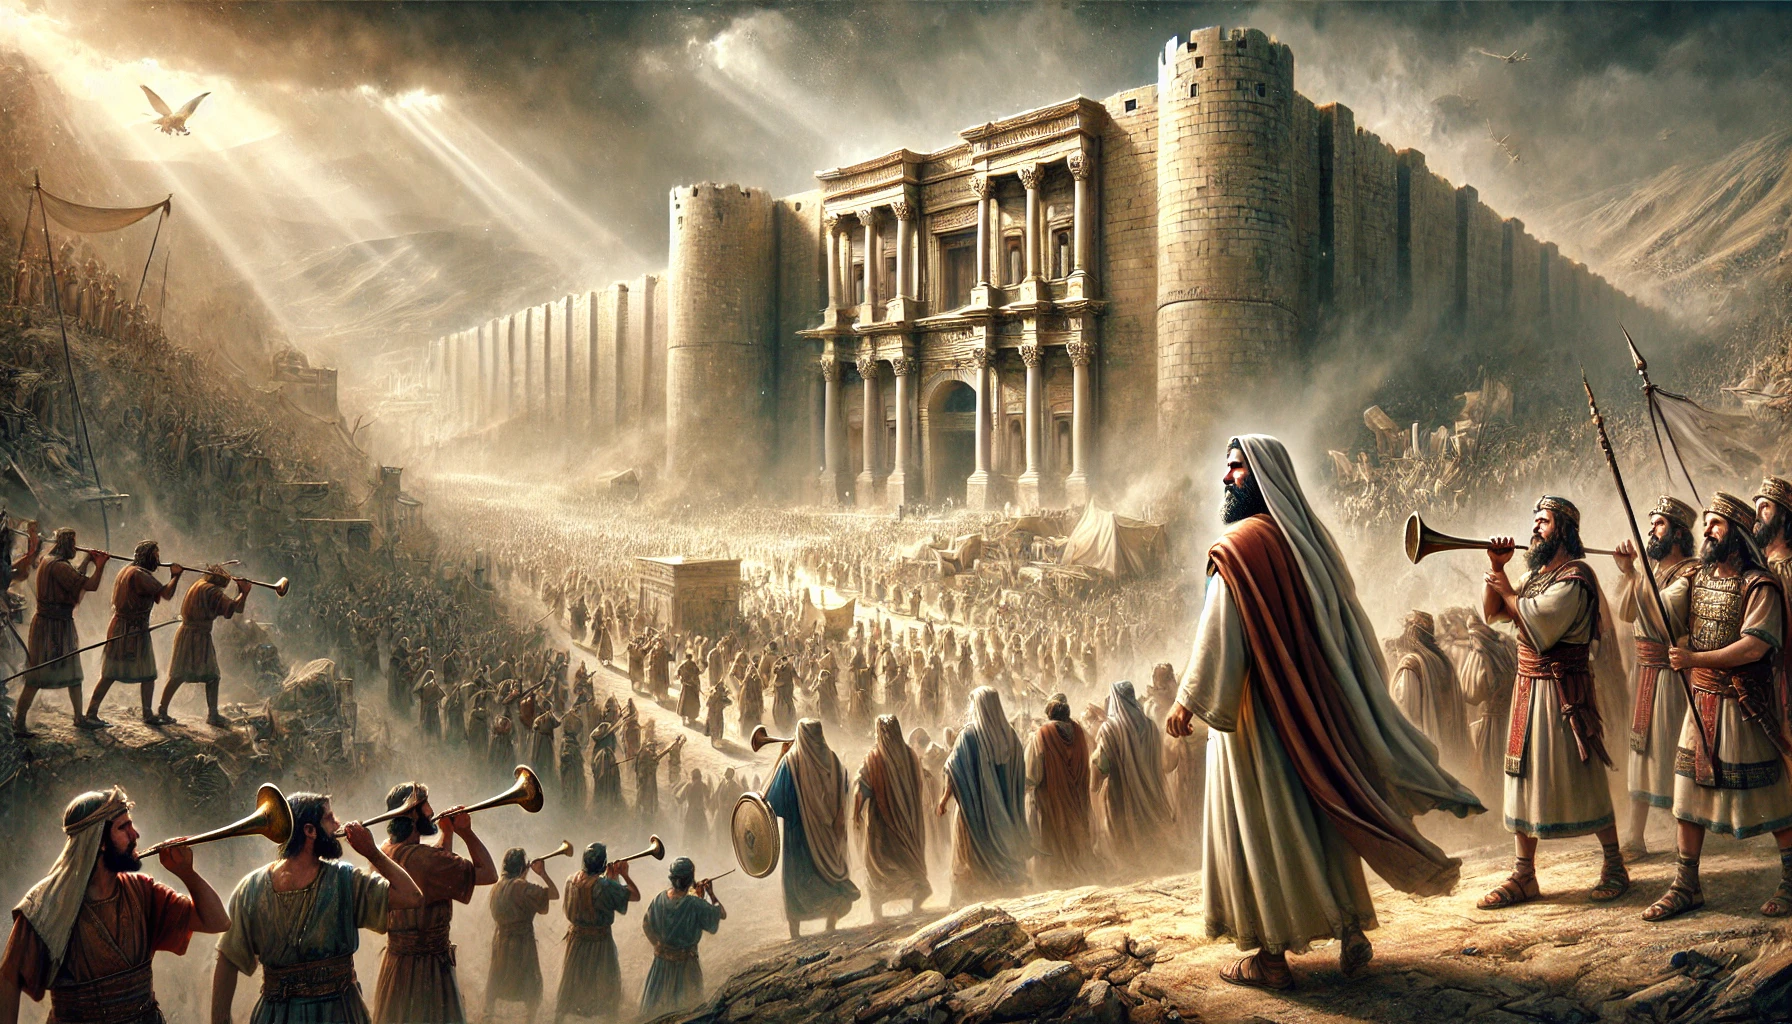
\includegraphics[width=0.7\linewidth]{graficas/josue.png}\\
	Josué y los Israelitas ante las murallas de Jericó\\
\end{center}




\section*{Capítulo 1 }
Preparativos para la conquista  
1:1 Aconteció después de la muerte de Moisés siervo de Jehová, que Jehová habló a Josué hijo de Nun, servidor de Moisés, diciendo:  
1:2 Mi siervo Moisés ha muerto; ahora, pues, levántate y pasa este Jordán, tú y todo este pueblo, a la tierra que yo les doy a los hijos de Israel.  
1:3 Yo os he entregado, como lo había dicho a Moisés, todo lugar que pisare la planta de vuestro pie.  
1:4 Desde el desierto y el Líbano hasta el gran río Eufrates, toda la tierra de los heteos hasta el gran mar donde se pone el sol, será vuestro territorio.  
1:5 Nadie te podrá hacer frente en todos los días de tu vida; como estuve con Moisés, estaré contigo; no te dejaré, ni te desampararé.  
1:6 Esfuérzate y sé valiente; porque tú repartirás a este pueblo por heredad la tierra de la cual juré a sus padres que la daría a ellos.  
1:7 Solamente esfuérzate y sé muy valiente, para cuidar de hacer conforme a toda la ley que mi siervo Moisés te mandó; no te apartes de ella ni a diestra ni a siniestra, para que seas prosperado en todas las cosas que emprendas.  
1:8 Nunca se apartará de tu boca este libro de la ley, sino que de día y de noche meditarás en él, para que guardes y hagas conforme a todo lo que en él está escrito; porque entonces harás prosperar tu camino, y todo te saldrá bien.  
1:9 Mira que te mando que te esfuerces y seas valiente; no temas ni desmayes, porque Jehová tu Dios estará contigo en dondequiera que vayas.  
1:10 Y Josué mandó a los oficiales del pueblo, diciendo:  
1:11 Pasad por en medio del campamento y mandad al pueblo, diciendo: Preparaos comida, porque dentro de tres días pasaréis el Jordán para entrar a poseer la tierra que Jehová vuestro Dios os da en posesión.  
1:12 También habló Josué a los rubenitas y gaditas y a la media tribu de Manasés, diciendo:  
1:13 Acordaos de la palabra que Moisés, siervo de Jehová, os mandó diciendo: Jehová vuestro Dios os ha dado reposo, y os ha dado esta tierra.  
1:14 Vuestras mujeres, vuestros niños y vuestros ganados quedarán en la tierra que Moisés os ha dado a este lado del Jordán; mas vosotros, todos los valientes y fuertes, pasaréis armados delante de vuestros hermanos, y les ayudaréis,  
1:15 hasta tanto que Jehová haya dado reposo a vuestros hermanos como a vosotros, y que ellos también posean la tierra que Jehová vuestro Dios les da; y después volveréis vosotros a la tierra de vuestra herencia, la cual Moisés siervo de Jehová os ha dado, a este lado del Jordán hacia donde nace el sol; y entraréis en posesión de ella. 
1:16 Entonces respondieron a Josué, diciendo: Nosotros haremos todas las cosas que nos has mandado, e iremos adondequiera que nos mandes.  
1:17 De la manera que obedecimos a Moisés en todas las cosas, así te obedeceremos a ti; solamente que Jehová tu Dios esté contigo, como estuvo con Moisés.  
1:18 Cualquiera que fuere rebelde a tu mandamiento, y no obedeciere a tus palabras en todas las cosas que le mandes, que muera; solamente que te esfuerces y seas valiente.  
\section*{Capítulo 2}
Josué envía espías a Jericó  

2:1 Josué hijo de Nun envió desde Sitim dos espías secretamente, diciéndoles: Andad, reconoced la tierra, y a Jericó. Y ellos fueron, y entraron en casa de una ramera que se llamaba Rahab, y posaron allí.  
2:2 Y fue dado aviso al rey de Jericó, diciendo: He aquí que hombres de los hijos de Israel han venido aquí esta noche para espiar la tierra.  
2:3 Entonces el rey de Jericó envió a decir a Rahab: Saca a los hombres que han venido a ti, y han entrado a tu casa; porque han venido para espiar toda la tierra.  
2:4 Pero la mujer había tomado a los dos hombres y los había escondido; y dijo: Es verdad que unos hombres vinieron a mí, pero no supe de dónde eran.  
2:5 Y cuando se iba a cerrar la puerta, siendo ya oscuro, esos hombres se salieron, y no sé a dónde han ido; seguidlos aprisa, y los alcanzaréis.  
2:6 Mas ella los había hecho subir al terrado, y los había escondido entre los manojos de lino que tenía puestos en el terrado.  
2:7 Y los hombres fueron tras ellos por el camino del Jordán, hasta los vados; y la puerta fue cerrada después que salieron los perseguidores.  
2:8 Antes que ellos se durmiesen, ella subió al terrado, y les dijo:  
2:9 Sé que Jehová os ha dado esta tierra; porque el temor de vosotros ha caído sobre nosotros, y todos los moradores del país ya han desmayado por causa de vosotros.  
2:10 Porque hemos oído que Jehová hizo secar las aguas del Mar Rojo delante de vosotros cuando salisteis de Egipto, y lo que habéis hecho a los dos reyes de los amorreos que estaban al otro lado del Jordán, a Sehón y a Og, a los cuales habéis destruido. 
2:11 Oyendo esto, ha desmayado nuestro corazón; ni ha quedado más aliento en hombre alguno por causa de vosotros, porque Jehová vuestro Dios es Dios arriba en los cielos y abajo en la tierra.  
2:12 Os ruego pues, ahora, que me juréis por Jehová, que como he hecho misericordia con vosotros, así la haréis vosotros con la casa de mi padre, de lo cual me daréis una señal segura;  
2:13 y que salvaréis la vida a mi padre y a mi madre, a mis hermanos y hermanas, y a todo lo que es suyo; y que libraréis nuestras vidas de la muerte.  
2:14 Ellos le respondieron: Nuestra vida responderá por la vuestra, si no denunciareis este asunto nuestro; y cuando Jehová nos haya dado la tierra, nosotros haremos contigo misericordia y verdad.  
2:15 Entonces ella los hizo descender con una cuerda por la ventana; porque su casa estaba en el muro de la ciudad, y ella vivía en el muro.  
2:16 Y les dijo: Marchaos al monte, para que los que fueron tras vosotros no os encuentren; y estad escondidos allí tres días, hasta que los que os siguen hayan vuelto; y después os iréis por vuestro camino.  
2:17 Y ellos le dijeron: Nosotros quedaremos libres de este juramento con que nos has juramentado.  
2:18 He aquí, cuando nosotros entremos en la tierra, tú atarás este cordón de grana a la ventana por la cual nos descolgaste; y reunirás en tu casa a tu padre y a tu madre, a tus hermanos y a toda la familia de tu padre.  
2:19 Cualquiera que saliere fuera de las puertas de tu casa, su sangre será sobre su cabeza, y nosotros sin culpa. Mas cualquiera que se estuviere en casa contigo, su sangre será sobre nuestra cabeza, si mano le tocare.  
2:20 Y si tú denunciares este nuestro asunto, nosotros quedaremos libres de este tu juramento con que nos has juramentado.  
2:21 Ella respondió: Sea así como habéis dicho. Luego los despidió, y se fueron; y ella ató el cordón de grana a la ventana.  
2:22 Y caminando ellos, llegaron al monte y estuvieron allí tres días, hasta que volvieron los que los perseguían; y los que los persiguieron buscaron por todo el camino, pero no los hallaron.  
2:23 Entonces volvieron los dos hombres; descendieron del monte, y pasaron, y vinieron a Josué hijo de Nun, y le contaron todas las cosas que les habían acontecido.  
2:24 Y dijeron a Josué: Jehová ha entregado toda la tierra en nuestras manos; y también todos los moradores del país desmayan delante de nosotros.  
\section*{Capítulo 3}
El paso del Jordán  

3:1 Josué se levantó de mañana, y él y todos los hijos de Israel partieron de Sitim y vinieron hasta el Jordán, y reposaron allí antes de pasarlo.  
3:2 Y después de tres días, los oficiales recorrieron el campamento,  
3:3 y mandaron al pueblo, diciendo: Cuando veáis el arca del pacto de Jehová vuestro Dios, y los levitas sacerdotes que la llevan, vosotros saldréis de vuestro lugar y marcharéis en pos de ella,  
3:4 a fin de que sepáis el camino por donde habéis de ir; por cuanto vosotros no habéis pasado antes de ahora por este camino. Pero entre vosotros y ella haya distancia como de dos mil codos; no os acercaréis a ella.  
3:5 Y Josué dijo al pueblo: Santificaos, porque Jehová hará mañana maravillas entre vosotros.  
3:6 Y habló Josué a los sacerdotes, diciendo: Tomad el arca del pacto, y pasad delante del pueblo. Y ellos tomaron el arca del pacto y fueron delante del pueblo.  
3:7 Entonces Jehová dijo a Josué: Desde este día comenzaré a engrandecerte delante de los ojos de todo Israel, para que entiendan que como estuve con Moisés, así estaré contigo.  
3:8 Tú, pues, mandarás a los sacerdotes que llevan el arca del pacto, diciendo: Cuando hayáis entrado hasta el borde del agua del Jordán, pararéis en el Jordán.  
3:9 Y Josué dijo a los hijos de Israel: Acercaos, y escuchad las palabras de Jehová vuestro Dios.  
3:10 Y añadió Josué: En esto conoceréis que el Dios viviente está en medio de vosotros, y que él echará de delante de vosotros al cananeo, al heteo, al heveo, al ferezeo, al gergeseo, al amorreo y al jebuseo.  
3:11 He aquí, el arca del pacto del Señor de toda la tierra pasará delante de vosotros en medio del Jordán.  
3:12 Tomad, pues, ahora doce hombres de las tribus de Israel, uno de cada tribu.  
3:13 Y cuando las plantas de los pies de los sacerdotes que llevan el arca de Jehová, Señor de toda la tierra, se asienten en las aguas del Jordán, las aguas del Jordán se dividirán; porque las aguas que vienen de arriba se detendrán en un montón.  
3:14 Y aconteció cuando partió el pueblo de sus tiendas para pasar el Jordán, con los sacerdotes delante del pueblo llevando el arca del pacto,  
3:15 cuando los que llevaban el arca entraron en el Jordán, y los pies de los sacerdotes que llevaban el arca fueron mojados a la orilla del agua (porque el Jordán suele desbordarse por todas sus orillas todo el tiempo de la siega),  
3:16 las aguas que venían de arriba se detuvieron como en un montón bien lejos de la ciudad de Adam, que está al lado de Saretán, y las que descendían al mar del Arabá, al Mar Salado, se acabaron, y fueron divididas; y el pueblo pasó en dirección de Jericó.  
3:17 Mas los sacerdotes que llevaban el arca del pacto de Jehová, estuvieron en seco, firmes en medio del Jordán, hasta que todo el pueblo hubo acabado de pasar el Jordán; y todo Israel pasó en seco.  
\section*{Capítulo 4}
Las doce piedras tomadas del Jordán  

4:1 Cuando toda la gente hubo acabado de pasar el Jordán, Jehová habló a Josué, diciendo:  
4:2 Tomad del pueblo doce hombres, uno de cada tribu,  
4:3 y mandadles, diciendo: Tomad de aquí de en medio del Jordán, del lugar donde están firmes los pies de los sacerdotes, doce piedras, las cuales pasaréis con vosotros, y levantadlas en el lugar donde habéis de pasar la noche.  
4:4 Entonces Josué llamó a los doce hombres a los cuales él había designado de entre los hijos de Israel, uno de cada tribu.  
4:5 Y les dijo Josué: Pasad delante del arca de Jehová vuestro Dios a la mitad del Jordán, y cada uno de vosotros tome una piedra sobre su hombro, conforme al número de las tribus de los hijos de Israel,  
4:6 para que esto sea señal entre vosotros; y cuando vuestros hijos preguntaren a sus padres mañana, diciendo: ¿Qué significan estas piedras?  
4:7 les responderéis: Que las aguas del Jordán fueron divididas delante del arca del pacto de Jehová; cuando ella pasó el Jordán, las aguas del Jordán se dividieron; y estas piedras servirán de monumento conmemorativo a los hijos de Israel para siempre.  
4:8 Y los hijos de Israel lo hicieron así como Josué les mandó: tomaron doce piedras de en medio del Jordán, como Jehová lo había dicho a Josué, conforme al número de las tribus de los hijos de Israel, y las pasaron al lugar donde acamparon, y las levantaron allí.  
4:9 Josué también levantó doce piedras en medio del Jordán, en el lugar donde estuvieron los pies de los sacerdotes que llevaban el arca del pacto; y han estado allí hasta hoy.  
4:10 Y los sacerdotes que llevaban el arca se pararon en medio del Jordán hasta que se hizo todo lo que Jehová había mandado a Josué que dijese al pueblo, conforme a todas las cosas que Moisés había mandado a Josué; y el pueblo se dio prisa y pasó.  
4:11 Y cuando todo el pueblo acabó de pasar, también pasó el arca de Jehová, y los sacerdotes, en presencia del pueblo.  
4:12 También los hijos de Rubén y los hijos de Gad y la media tribu de Manasés pasaron armados delante de los hijos de Israel, según Moisés les había dicho;  
4:13 como cuarenta mil hombres armados, listos para la guerra, pasaron hacia la llanura de Jericó delante de Jehová.  
4:14 En aquel día Jehová engrandeció a Josué a los ojos de todo Israel; y le temieron, como habían temido a Moisés, todos los días de su vida.  
4:15 Luego Jehová habló a Josué, diciendo:  
4:16 Manda a los sacerdotes que llevan el arca del testimonio, que suban del Jordán.  
4:17 Y Josué mandó a los sacerdotes, diciendo: Subid del Jordán.  
4:18 Y aconteció que cuando los sacerdotes que llevaban el arca del pacto de Jehová subieron de en medio del Jordán, y las plantas de los pies de los sacerdotes estuvieron en lugar seco, las aguas del Jordán se volvieron a su lugar, corriendo como antes sobre todos sus bordes.  
4:19 Y el pueblo subió del Jordán el día diez del mes primero, y acamparon en Gilgal, al lado oriental de Jericó.  
4:20 Y Josué erigió en Gilgal las doce piedras que habían traído del Jordán.  
4:21 Y habló a los hijos de Israel, diciendo: Cuando mañana preguntaren vuestros hijos a sus padres, y dijeren: ¿Qué significan estas piedras?  
4:22 declararéis a vuestros hijos, diciendo: Israel pasó en seco por este Jordán.  
4:23 Porque Jehová vuestro Dios secó las aguas del Jordán delante de vosotros, hasta que habíais pasado, a la manera que Jehová vuestro Dios lo había hecho en el Mar Rojo, el cual secó delante de nosotros hasta que pasamos;  
4:24 para que todos los pueblos de la tierra conozcan que la mano de Jehová es poderosa; para que temáis a Jehová vuestro Dios todos los días.  
\section*{Capítulo 5 }
La circuncisión y la pascua en Gilgal  

5:1 Cuando todos los reyes de los amorreos que estaban al otro lado del Jordán al occidente, y todos los reyes de los cananeos que estaban cerca del mar, oyeron cómo Jehová había secado las aguas del Jordán delante de los hijos de Israel hasta que hubieron pasado, desfalleció su corazón, y no hubo más aliento en ellos delante de los hijos de Israel.  
5:2 En aquel tiempo Jehová dijo a Josué: Hazte cuchillos afilados, y vuelve a circuncidar la segunda vez a los hijos de Israel.  
5:3 Y Josué se hizo cuchillos afilados, y circuncidó a los hijos de Israel en el collado de Aralot.  
5:4 Esta es la causa por la cual Josué los circuncidó: Todo el pueblo que había salido de Egipto, los varones, todos los hombres de guerra, habían muerto en el desierto, por el camino, después que salieron de Egipto.  
5:5 Pues todos los del pueblo que habían salido, estaban circuncidados; mas todo el pueblo que había nacido en el desierto, por el camino, después que hubieron salido de Egipto, no estaba circuncidado.  
5:6 Porque los hijos de Israel anduvieron por el desierto cuarenta años, hasta que todos los hombres de guerra que habían salido de Egipto fueron consumidos, por cuanto no obedecieron a la voz de Jehová; por lo cual Jehová les juró que no les dejaría ver la tierra de la cual Jehová había jurado a sus padres que nos la daría, tierra que fluye leche y miel. 
5:7 A los hijos de ellos, que él había hecho suceder en su lugar, Josué los circuncidó; pues eran incircuncisos, porque no habían sido circuncidados por el camino.  
5:8 Y cuando acabaron de circuncidar a toda la gente, se quedaron en el mismo lugar en el campamento, hasta que sanaron.  
5:9 Y Jehová dijo a Josué: Hoy he quitado de vosotros el oprobio de Egipto; por lo cual el nombre de aquel lugar fue llamado Gilgal, hasta hoy.  
5:10 Y los hijos de Israel acamparon en Gilgal, y celebraron la pascua a los catorce días del mes, por la tarde, en los llanos de Jericó.  
5:11 Al otro día de la pascua comieron del fruto de la tierra, los panes sin levadura, y en el mismo día espigas nuevas tostadas.  
5:12 Y el maná cesó el día siguiente, desde que comenzaron a comer del fruto de la tierra; y los hijos de Israel nunca más tuvieron maná, sino que comieron de los frutos de la tierra de Canaán aquel año.  
Josué y el varón con la espada desenvainada  
5:13 Estando Josué cerca de Jericó, alzó sus ojos y vio un varón que estaba delante de él, el cual tenía una espada desenvainada en su mano. Y Josué, yendo hacia él, le dijo: ¿Eres de los nuestros, o de nuestros enemigos?  
5:14 El respondió: No; mas como Príncipe del ejército de Jehová he venido ahora. Entonces Josué, postrándose sobre su rostro en tierra, le adoró; y le dijo: ¿Qué dice mi Señor a su siervo?  
5:15 Y el Príncipe del ejército de Jehová respondió a Josué: Quita el calzado de tus pies, porque el lugar donde estás es santo. Y Josué así lo hizo.  
\section*{Capítulo 6 }
La toma de Jericó  

6:1 Ahora, Jericó estaba cerrada, bien cerrada, a causa de los hijos de Israel; nadie entraba ni salía.  
6:2 Mas Jehová dijo a Josué: Mira, yo he entregado en tu mano a Jericó y a su rey, con sus varones de guerra.  
6:3 Rodearéis, pues, la ciudad todos los hombres de guerra, yendo alrededor de la ciudad una vez; y esto haréis durante seis días.  
6:4 Y siete sacerdotes llevarán siete bocinas de cuernos de carnero delante del arca; y al séptimo día daréis siete vueltas a la ciudad, y los sacerdotes tocarán las bocinas.  
6:5 Y cuando toquen prolongadamente el cuerno de carnero, así que oigáis el sonido de la bocina, todo el pueblo gritará a gran voz, y el muro de la ciudad caerá; entonces subirá el pueblo, cada uno derecho hacia adelante.  
6:6 Llamando, pues, Josué hijo de Nun a los sacerdotes, les dijo: Llevad el arca del pacto, y siete sacerdotes lleven bocinas de cuerno de carnero delante del arca de Jehová.  
6:7 Y dijo al pueblo: Pasad, y rodead la ciudad; y los que están armados pasarán delante del arca de Jehová.  
6:8 Y así que Josué hubo hablado al pueblo, los siete sacerdotes, llevando las siete bocinas de cuerno de carnero, pasaron delante del arca de Jehová, y tocaron las bocinas; y el arca del pacto de Jehová los seguía.  
6:9 Y los hombres armados iban delante de los sacerdotes que tocaban las bocinas, y la retaguardia iba tras el arca, mientras las bocinas sonaban continuamente.  
6:10 Y Josué mandó al pueblo, diciendo: Vosotros no gritaréis, ni se oirá vuestra voz, ni saldrá palabra de vuestra boca, hasta el día que yo os diga: Gritad; entonces gritaréis.  
6:11 Así que él hizo que el arca de Jehová diera una vuelta alrededor de la ciudad, y volvieron luego al campamento, y allí pasaron la noche.  
6:12 Y Josué se levantó de mañana, y los sacerdotes tomaron el arca de Jehová.  
6:13 Y los siete sacerdotes, llevando las siete bocinas de cuerno de carnero, fueron delante del arca de Jehová, andando siempre y tocando las bocinas; y los hombres armados iban delante de ellos, y la retaguardia iba tras el arca de Jehová, mientras las bocinas tocaban continuamente.  
6:14 Así dieron otra vuelta a la ciudad el segundo día, y volvieron al campamento; y de esta manera hicieron durante seis días.  
6:15 Al séptimo día se levantaron al despuntar el alba, y dieron vuelta a la ciudad de la misma manera siete veces; solamente este día dieron vuelta alrededor de ella siete veces.  
6:16 Y cuando los sacerdotes tocaron las bocinas la séptima vez, Josué dijo al pueblo: Gritad, porque Jehová os ha entregado la ciudad.  
6:17 Y será la ciudad anatema a Jehová, con todas las cosas que están en ella; solamente Rahab la ramera vivirá, con todos los que estén en casa con ella, por cuanto escondió a los mensajeros que enviamos.  
6:18 Pero vosotros guardaos del anatema; ni toquéis, ni toméis alguna cosa del anatema, no sea que hagáis anatema el campamento de Israel, y lo turbéis.  
6:19 Mas toda la plata y el oro, y los utensilios de bronce y de hierro, sean consagrados a Jehová, y entren en el tesoro de Jehová.  
6:20 Entonces el pueblo gritó, y los sacerdotes tocaron las bocinas; y aconteció que cuando el pueblo hubo oído el sonido de la bocina, gritó con gran vocerío, y el muro se derrumbó. El pueblo subió luego a la ciudad, cada uno derecho hacia adelante, y la tomaron.  
6:21 Y destruyeron a filo de espada todo lo que en la ciudad había; hombres y mujeres, jóvenes y viejos, hasta los bueyes, las ovejas, y los asnos.  
6:22 Mas Josué dijo a los dos hombres que habían reconocido la tierra: Entrad en casa de la mujer ramera, y haced salir de allí a la mujer y a todo lo que fuere suyo, como lo jurasteis.  
6:23 Y los espías entraron y sacaron a Rahab, a su padre, a su madre, a sus hermanos y todo lo que era suyo; y también sacaron a toda su parentela, y los pusieron fuera del campamento de Israel.  
6:24 Y consumieron con fuego la ciudad, y todo lo que en ella había; solamente pusieron en el tesoro de la casa de Jehová la plata y el oro, y los utensilios de bronce y de hierro.  
6:25 Mas Josué salvó la vida a Rahab la ramera, y a la casa de su padre, y a todo lo que ella tenía; y habitó ella entre los israelitas hasta hoy, por cuanto escondió a los mensajeros que Josué había enviado a reconocer a Jericó. 
6:26 En aquel tiempo hizo Josué un juramento, diciendo: Maldito delante de Jehová el hombre que se levantare y reedificare esta ciudad de Jericó. Sobre su primogénito eche los cimientos de ella, y sobre su hijo menor asiente sus puertas. 
6:27 Estaba, pues, Jehová con Josué, y su nombre se divulgó por toda la tierra.  
\section*{Capítulo 7 }
El pecado de Acán  

7:1 Pero los hijos de Israel cometieron una prevaricación en cuanto al anatema; porque Acán hijo de Carmi, hijo de Zabdi, hijo de Zera, de la tribu de Judá, tomó del anatema; y la ira de Jehová se encendió contra los hijos de Israel.  
7:2 Después Josué envió hombres desde Jericó a Hai, que estaba junto a Bet-avén hacia el oriente de Bet-el; y les habló diciendo: Subid y reconoced la tierra. Y ellos subieron y reconocieron a Hai.  
7:3 Y volviendo a Josué, le dijeron: No suba todo el pueblo, sino suban como dos mil o tres mil hombres, y tomarán a Hai; no fatigues a todo el pueblo yendo allí, porque son pocos.  
7:4 Y subieron allá del pueblo como tres mil hombres, los cuales huyeron delante de los de Hai.  
7:5 Y los de Hai mataron de ellos a unos treinta y seis hombres, y los siguieron desde la puerta hasta Sebarim, y los derrotaron en la bajada; por lo cual el corazón del pueblo desfalleció y vino a ser como agua.  
7:6 Entonces Josué rompió sus vestidos, y se postró en tierra sobre su rostro delante del arca de Jehová hasta caer la tarde, él y los ancianos de Israel; y echaron polvo sobre sus cabezas.  
7:7 Y Josué dijo: ¡Ah, Señor Jehová! ¿Por qué hiciste pasar a este pueblo el Jordán, para entregarnos en las manos de los amorreos, para que nos destruyan? ¡Ojalá nos hubiéramos quedado al otro lado del Jordán!  
7:8 ¡Ay, Señor! ¿qué diré, ya que Israel ha vuelto la espalda delante de sus enemigos?  
7:9 Porque los cananeos y todos los moradores de la tierra oirán, y nos rodearán, y borrarán nuestro nombre de sobre la tierra; y entonces, ¿qué harás tú a tu grande nombre?  
7:10 Y Jehová dijo a Josué: Levántate; ¿por qué te postras así sobre tu rostro?  
7:11 Israel ha pecado, y aun han quebrantado mi pacto que yo les mandé; y también han tomado del anatema, y hasta han hurtado, han mentido, y aun lo han guardado entre sus enseres.  
7:12 Por esto los hijos de Israel no podrán hacer frente a sus enemigos, sino que delante de sus enemigos volverán la espalda, por cuanto han venido a ser anatema; ni estaré más con vosotros, si no destruyereis el anatema de en medio de vosotros.  
7:13 Levántate, santifica al pueblo, y di: Santificaos para mañana; porque Jehová el Dios de Israel dice así: Anatema hay en medio de ti, Israel; no podrás hacer frente a tus enemigos, hasta que hayáis quitado el anatema de en medio de vosotros.  
7:14 Os acercaréis, pues, mañana por vuestras tribus; y la tribu que Jehová tomare, se acercará por sus familias; y la familia que Jehová tomare, se acercará por sus casas; y la casa que Jehová tomare, se acercará por los varones;  
7:15 y el que fuere sorprendido en el anatema, será quemado, él y todo lo que tiene, por cuanto ha quebrantado el pacto de Jehová, y ha cometido maldad en Israel.  
7:16 Josué, pues, levantándose de mañana, hizo acercar a Israel por sus tribus; y fue tomada la tribu de Judá.  
7:17 Y haciendo acercar a la tribu de Judá, fue tomada la familia de los de Zera; y haciendo luego acercar a la familia de los de Zera por los varones, fue tomado Zabdi.  
7:18 Hizo acercar su casa por los varones, y fue tomado Acán hijo de Carmi, hijo de Zabdi, hijo de Zera, de la tribu de Judá.  
7:19 Entonces Josué dijo a Acán: Hijo mío, da gloria a Jehová el Dios de Israel, y dale alabanza, y declárame ahora lo que has hecho; no me lo encubras.  
7:20 Y Acán respondió a Josué diciendo: Verdaderamente yo he pecado contra Jehová el Dios de Israel, y así y así he hecho.  
7:21 Pues vi entre los despojos un manto babilónico muy bueno, y doscientos siclos de plata, y un lingote de oro de peso de cincuenta siclos, lo cual codicié y tomé; y he aquí que está escondido bajo tierra en medio de mi tienda, y el dinero debajo de ello.  
7:22 Josué entonces envió mensajeros, los cuales fueron corriendo a la tienda; y he aquí estaba escondido en su tienda, y el dinero debajo de ello.  
7:23 Y tomándolo de en medio de la tienda, lo trajeron a Josué y a todos los hijos de Israel, y lo pusieron delante de Jehová. 
7:24 Entonces Josué, y todo Israel con él, tomaron a Acán hijo de Zera, el dinero, el manto, el lingote de oro, sus hijos, sus hijas, sus bueyes, sus asnos, sus ovejas, su tienda y todo cuanto tenía, y lo llevaron todo al valle de Acor.  
7:25 Y le dijo Josué: ¿Por qué nos has turbado? Túrbete Jehová en este día. Y todos los israelitas los apedrearon, y los quemaron después de apedrearlos.  
7:26 Y levantaron sobre él un gran montón de piedras, que permanece hasta hoy. Y Jehová se volvió del ardor de su ira. Y por esto aquel lugar se llama el Valle de Acor, hasta hoy.  
\section*{Capítulo 8}
Toma y destrucción de Hai  

8:1 Jehová dijo a Josué: No temas ni desmayes; toma contigo toda la gente de guerra, y levántate y sube a Hai. Mira, yo he entregado en tu mano al rey de Hai, a su pueblo, a su ciudad y a su tierra.  
8:2 Y harás a Hai y a su rey como hiciste a Jericó y a su rey; sólo que sus despojos y sus bestias tomaréis para vosotros. Pondrás, pues, emboscadas a la ciudad detrás de ella.  
8:3 Entonces se levantaron Josué y toda la gente de guerra, para subir contra Hai; y escogió Josué treinta mil hombres fuertes, los cuales envió de noche.  
8:4 Y les mandó, diciendo: Atended, pondréis emboscada a la ciudad detrás de ella; no os alejaréis mucho de la ciudad, y estaréis todos dispuestos.  
8:5 Y yo y todo el pueblo que está conmigo nos acercaremos a la ciudad; y cuando salgan ellos contra nosotros, como hicieron antes, huiremos delante de ellos.  
8:6 Y ellos saldrán tras nosotros, hasta que los alejemos de la ciudad; porque dirán: Huyen de nosotros como la primera vez. Huiremos, pues, delante de ellos.  
8:7 Entonces vosotros os levantaréis de la emboscada y tomaréis la ciudad; pues Jehová vuestro Dios la entregará en vuestras manos.  
8:8 Y cuando la hayáis tomado, le prenderéis fuego. Haréis conforme a la palabra de Jehová; mirad que os lo he mandado.  
8:9 Entonces Josué los envió; y ellos se fueron a la emboscada, y se pusieron entre Bet-el y Hai, al occidente de Hai; y Josué se quedó aquella noche en medio del pueblo.  
8:10 Levantándose Josué muy de mañana, pasó revista al pueblo, y subió él, con los ancianos de Israel, delante del pueblo contra Hai.  
8:11 Y toda la gente de guerra que con él estaba, subió y se acercó, y llegaron delante de la ciudad, y acamparon al norte de Hai; y el valle estaba entre él y Hai.  
8:12 Y tomó como cinco mil hombres, y los puso en emboscada entre Bet-el y Hai, al occidente de la ciudad.  
8:13 Así dispusieron al pueblo: todo el campamento al norte de la ciudad, y su emboscada al occidente de la ciudad, y Josué avanzó aquella noche hasta la mitad del valle.  
8:14 Y aconteció que viéndolo el rey de Hai, él y su pueblo se apresuraron y madrugaron; y al tiempo señalado, los hombres de la ciudad salieron al encuentro de Israel para combatir, frente al Arabá, no sabiendo que estaba puesta emboscada a espaldas de la ciudad.  
8:15 Entonces Josué y todo Israel se fingieron vencidos y huyeron delante de ellos por el camino del desierto.  
8:16 Y todo el pueblo que estaba en Hai se juntó para seguirles; y siguieron a Josué, siendo así alejados de la ciudad. 
8:17 Y no quedó hombre en Hai ni en Bet-el, que no saliera tras de Israel; y por seguir a Israel dejaron la ciudad abierta.  
8:18 Entonces Jehová dijo a Josué: Extiende la lanza que tienes en tu mano hacia Hai, porque yo la entregaré en tu mano. Y Josué extendió hacia la ciudad la lanza que en su mano tenía.  
8:19 Y levantándose prontamente de su lugar los que estaban en la emboscada, corrieron luego que él alzó su mano, y vinieron a la ciudad, y la tomaron, y se apresuraron a prenderle fuego.  
8:20 Y los hombres de Hai volvieron el rostro, y al mirar, he aquí que el humo de la ciudad subía al cielo, y no pudieron huir ni a una parte ni a otra, porque el pueblo que iba huyendo hacia el desierto se volvió contra los que les seguían.  
8:21 Josué y todo Israel, viendo que los de la emboscada habían tomado la ciudad, y que el humo de la ciudad subía, se volvieron y atacaron a los de Hai.  
8:22 Y los otros salieron de la ciudad a su encuentro, y así fueron encerrados en medio de Israel, los unos por un lado, y los otros por el otro. Y los hirieron hasta que no quedó ninguno de ellos que escapase.  
8:23 Pero tomaron vivo al rey de Hai, y lo trajeron a Josué.  
8:24 Y cuando los israelitas acabaron de matar a todos los moradores de Hai en el campo y en el desierto a donde los habían perseguido, y todos habían caído a filo de espada hasta ser consumidos, todos los israelitas volvieron a Hai, y también la hirieron a filo de espada.  
8:25 Y el número de los que cayeron aquel día, hombres y mujeres, fue de doce mil, todos los de Hai.  
8:26 Porque Josué no retiró su mano que había extendido con la lanza, hasta que hubo destruido por completo a todos los moradores de Hai.  
8:27 Pero los israelitas tomaron para sí las bestias y los despojos de la ciudad, conforme a la palabra de Jehová que le había mandado a Josué.  
8:28 Y Josué quemó a Hai y la redujo a un montón de escombros, asolada para siempre hasta hoy.  
8:29 Y al rey de Hai lo colgó de un madero hasta caer la noche; y cuando el sol se puso, mandó Josué que quitasen del madero su cuerpo, y lo echasen a la puerta de la ciudad; y levantaron sobre él un gran montón de piedras, que permanece hasta hoy.  
Lectura de la ley en el Monte Ebal  
8:30 Entonces Josué edificó un altar a Jehová Dios de Israel en el monte Ebal,  
8:31 como Moisés siervo de Jehová lo había mandado a los hijos de Israel, como está escrito en el libro de la ley de Moisés, un altar de piedras enteras sobre las cuales nadie alzó hierro; y ofrecieron sobre él holocaustos a Jehová, y sacrificaron ofrendas de paz.  
8:32 También escribió allí sobre las piedras una copia de la ley de Moisés, la cual escribió delante de los hijos de Israel. 
8:33 Y todo Israel, con sus ancianos, oficiales y jueces, estaba de pie a uno y otro lado del arca, en presencia de los sacerdotes levitas que llevaban el arca del pacto de Jehová, así los extranjeros como los naturales. La mitad de ellos estaba hacia el monte Gerizim, y la otra mitad hacia el monte Ebal, de la manera que Moisés, siervo de Jehová, lo había mandado antes, para que bendijesen primeramente al pueblo de Israel.  
8:34 Después de esto, leyó todas las palabras de la ley, las bendiciones y las maldiciones, conforme a todo lo que está escrito en el libro de la ley.  
8:35 No hubo palabra alguna de todo cuanto mandó Moisés, que Josué no hiciese leer delante de toda la congregación de Israel, y de las mujeres, de los niños, y de los extranjeros que moraban entre ellos. 
\section*{Capítulo 9 }
Astucia de los gabaonitas  

9:1 Cuando oyeron estas cosas todos los reyes que estaban a este lado del Jordán, así en las montañas como en los llanos, y en toda la costa del Mar Grande delante del Líbano, los heteos, amorreos, cananeos, ferezeos, heveos y jebuseos,  
9:2 se concertaron para pelear contra Josué e Israel.  
9:3 Mas los moradores de Gabaón, cuando oyeron lo que Josué había hecho a Jericó y a Hai,  
9:4 usaron de astucia; pues fueron y se fingieron embajadores, y tomaron sacos viejos sobre sus asnos, y cueros viejos de vino, rotos y remendados,  
9:5 y zapatos viejos y recosidos en sus pies, con vestidos viejos sobre sí; y todo el pan que traían para el camino era seco y mohoso.  
9:6 Y vinieron a Josué al campamento en Gilgal, y le dijeron a él y a los de Israel: Nosotros venimos de tierra muy lejana; haced, pues, ahora alianza con nosotros.  
9:7 Y los de Israel respondieron a los heveos: Quizás habitáis en medio de nosotros. ¿Cómo, pues, podremos hacer alianza con vosotros?  
9:8 Ellos respondieron a Josué: Nosotros somos tus siervos. Y Josué les dijo: ¿Quiénes sois vosotros, y de dónde venís?  
9:9 Y ellos respondieron: Tus siervos han venido de tierra muy lejana, por causa del nombre de Jehová tu Dios; porque hemos oído su fama, y todo lo que hizo en Egipto,  
9:10 y todo lo que hizo a los dos reyes de los amorreos que estaban al otro lado del Jordán: a Sehón rey de Hesbón, y a Og rey de Basán, que estaba en Astarot. 
9:11 Por lo cual nuestros ancianos y todos los moradores de nuestra tierra nos dijeron: Tomad en vuestras manos provisión para el camino, e id al encuentro de ellos, y decidles: Nosotros somos vuestros siervos; haced ahora alianza con nosotros.  
9:12 Este nuestro pan lo tomamos caliente de nuestras casas para el camino el día que salimos para venir a vosotros; y helo aquí ahora ya seco y mohoso.  
9:13 Estos cueros de vino también los llenamos nuevos; helos aquí ya rotos; también estos nuestros vestidos y nuestros zapatos están ya viejos a causa de lo muy largo del camino.  
9:14 Y los hombres de Israel tomaron de la provisiones de ellos, y no consultaron a Jehová.  
9:15 Y Josué hizo paz con ellos, y celebró con ellos alianza concediéndoles la vida; y también lo juraron los príncipes de la congregación.  
9:16 Pasados tres días después que hicieron alianza con ellos, oyeron que eran sus vecinos, y que habitaban en medio de ellos.  
9:17 Y salieron los hijos de Israel, y al tercer día llegaron a las ciudades de ellos; y sus ciudades eran Gabaón, Cafira, Beerot y Quiriat-jearim.  
9:18 Y no los mataron los hijos de Israel, por cuanto los príncipes de la congregación les habían jurado por Jehová el Dios de Israel. Y toda la congregación murmuraba contra los príncipes.  
9:19 Mas todos los príncipes respondieron a toda la congregación: Nosotros les hemos jurado por Jehová Dios de Israel; por tanto, ahora no les podemos tocar.  
9:20 Esto haremos con ellos: les dejaremos vivir, para que no venga ira sobre nosotros por causa del juramento que les hemos hecho.  
9:21 Dijeron, pues, de ellos los príncipes: Dejadlos vivir; y fueron constituidos leñadores y aguadores para toda la congregación, concediéndoles la vida, según les habían prometido los príncipes.  
9:22 Y llamándolos Josué, les habló diciendo: ¿Por qué nos habéis engañado, diciendo: Habitamos muy lejos de vosotros, siendo así que moráis en medio de nosotros?  
9:23 Ahora, pues, malditos sois, y no dejará de haber de entre vosotros siervos, y quien corte la leña y saque el agua para la casa de mi Dios.  
9:24 Y ellos respondieron a Josué y dijeron: Como fue dado a entender a tus siervos que Jehová tu Dios había mandado a Moisés su siervo que os había de dar toda la tierra, y que había de destruir a todos los moradores de la tierra delante de vosotros, por esto temimos en gran manera por nuestras vidas a causa de vosotros, e hicimos esto.  
9:25 Ahora, pues, henos aquí en tu mano; lo que te pareciere bueno y recto hacer de nosotros, hazlo.  
9:26 Y él lo hizo así con ellos; pues los libró de la mano de los hijos de Israel, y no los mataron.  
9:27 Y Josué los destinó aquel día a ser leñadores y aguadores para la congregación, y para el altar de Jehová en el lugar que Jehová eligiese, lo que son hasta hoy.  
\section*{Capítulo 10}
Derrota de los amorreos  

10:1 Cuando Adonisedec rey de Jerusalén oyó que Josué había tomado a Hai, y que la había asolado (como había hecho a Jericó y a su rey, así hizo a Hai y a su rey), y que los moradores de Gabaón habían hecho paz con los israelitas, y que estaban entre ellos,  
10:2 tuvo gran temor; porque Gabaón era una gran ciudad, como una de las ciudades reales, y mayor que Hai, y todos sus hombres eran fuertes.  
10:3 Por lo cual Adonisedec rey de Jerusalén envió a Hoham rey de Hebrón, a Piream rey de Jarmut, a Jafía rey de Laquis y a Debir rey de Eglón, diciendo:  
10:4 Subid a mí y ayudadme, y combatamos a Gabaón; porque ha hecho paz con Josué y con los hijos de Israel.  
10:5 Y cinco reyes de los amorreos, el rey de Jerusalén, el rey de Hebrón, el rey de Jarmut, el rey de Laquis y el rey de Eglón, se juntaron y subieron, ellos con todos sus ejércitos, y acamparon cerca de Gabaón, y pelearon contra ella.  
10:6 Entonces los moradores de Gabaón enviaron a decir a Josué al campamento en Gilgal: No niegues ayuda a tus siervos; sube prontamente a nosotros para defendernos y ayudarnos; porque todos los reyes de los amorreos que habitan en las montañas se han unido contra nosotros.  
10:7 Y subió Josué de Gilgal, él y todo el pueblo de guerra con él, y todos los hombres valientes.  
10:8 Y Jehová dijo a Josué: No tengas temor de ellos; porque yo los he entregado en tu mano, y ninguno de ellos prevalecerá delante de ti.  
10:9 Y Josué vino a ellos de repente, habiendo subido toda la noche desde Gilgal.  
10:10 Y Jehová los llenó de consternación delante de Israel, y los hirió con gran mortandad en Gabaón; y los siguió por el camino que sube a Bet-horón, y los hirió hasta Azeca y Maceda.  
10:11 Y mientras iban huyendo de los israelitas, a la bajada de Bet-horón, Jehová arrojó desde el cielo grandes piedras sobre ellos hasta Azeca, y murieron; y fueron más los que murieron por las piedras del granizo, que los que los hijos de Israel mataron a espada.  
10:12 Entonces Josué habló a Jehová el día en que Jehová entregó al amorreo delante de los hijos de Israel, y dijo en presencia de los israelitas:  
Sol, detente en Gabaón;  
Y tú, luna, en el valle de Ajalón. 
10:13 Y el sol se detuvo y la luna se paró,  
Hasta que la gente se hubo vengado de sus enemigos.  
¿No está escrito esto en el libro de Jaser? Y el sol se paró en medio del cielo, y no se apresuró a ponerse casi un día entero.  
10:14 Y no hubo día como aquel, ni antes ni después de él, habiendo atendido Jehová a la voz de un hombre; porque Jehová peleaba por Israel.  
10:15 Y Josué, y todo Israel con él, volvió al campamento en Gilgal.  
10:16 Y los cinco reyes huyeron, y se escondieron en una cueva en Maceda.  
10:17 Y fue dado aviso a Josué que los cinco reyes habían sido hallados escondidos en una cueva en Maceda.  
10:18 Entonces Josué dijo: Rodad grandes piedras a la entrada de la cueva, y poned hombres junto a ella para que los guarden;  
10:19 y vosotros no os detengáis, sino seguid a vuestros enemigos, y heridles la retaguardia, sin dejarles entrar en sus ciudades; porque Jehová vuestro Dios los ha entregado en vuestra mano.  
10:20 Y aconteció que cuando Josué y los hijos de Israel acabaron de herirlos con gran mortandad hasta destruirlos, los que quedaron de ellos se metieron en las ciudades fortificadas.  
10:21 Todo el pueblo volvió sano y salvo a Josué, al campamento en Maceda; no hubo quien moviese su lengua contra ninguno de los hijos de Israel.  
10:22 Entonces dijo Josué: Abrid la entrada de la cueva, y sacad de ella a esos cinco reyes.  
10:23 Y lo hicieron así, y sacaron de la cueva a aquellos cinco reyes: al rey de Jerusalén, al rey de Hebrón, al rey de Jarmut, al rey de Laquis y al rey de Eglón.  
10:24 Y cuando los hubieron llevado a Josué, llamó Josué a todos los varones de Israel, y dijo a los principales de la gente de guerra que habían venido con él: Acercaos, y poned vuestros pies sobre los cuellos de estos reyes. Y ellos se acercaron y pusieron sus pies sobre los cuellos de ellos.  
10:25 Y Josué les dijo: No temáis, ni os atemoricéis; sed fuertes y valientes, porque así hará Jehová a todos vuestros enemigos contra los cuales peleáis.  
10:26 Y después de esto Josué los hirió y los mató, y los hizo colgar en cinco maderos; y quedaron colgados en los maderos hasta caer la noche.  
10:27 Y cuando el sol se iba a poner, mandó Josué que los quitasen de los maderos, y los echasen en la cueva donde se habían escondido; y pusieron grandes piedras a la entrada de la cueva, las cuales permanecen hasta hoy.  
10:28 En aquel mismo día tomó Josué a Maceda, y la hirió a filo de espada, y mató a su rey; por completo los destruyó, con todo lo que en ella tenía vida, sin dejar nada; e hizo al rey de Maceda como había hecho al rey de Jericó.  
10:29 Y de Maceda pasó Josué, y todo Israel con él, a Libna; y peleó contra Libna;  
10:30 y Jehová la entregó también a ella y a su rey en manos de Israel; y la hirió a filo de espada, con todo lo que en ella tenía vida, sin dejar nada; e hizo a su rey de la manera como había hecho al rey de Jericó.  
10:31 Y Josué, y todo Israel con él, pasó de Libna a Laquis, y acampó cerca de ella, y la combatió;  
10:32 y Jehová entregó a Laquis en mano de Israel, y la tomó al día siguiente, y la hirió a filo de espada, con todo lo que en ella tenía vida, así como había hecho en Libna.  
10:33 Entonces Horam rey de Gezer subió en ayuda de Laquis; mas a él y a su pueblo destruyó Josué, hasta no dejar a ninguno de ellos.  
10:34 De Laquis pasó Josué, y todo Israel con él, a Eglón; y acamparon cerca de ella, y la combatieron;  
10:35 y la tomaron el mismo día, y la hirieron a filo de espada; y aquel día mató a todo lo que en ella tenía vida, como había hecho en Laquis.  
10:36 Subió luego Josué, y todo Israel con él, de Eglón a Hebrón, y la combatieron.  
10:37 Y tomándola, la hirieron a filo de espada, a su rey y a todas sus ciudades, con todo lo que en ella tenía vida, sin dejar nada; como había hecho a Eglón, así la destruyeron con todo lo que en ella tenía vida.  
10:38 Después volvió Josué, y todo Israel con él, sobre Debir, y combatió contra ella;  
10:39 y la tomó, y a su rey, y a todas sus ciudades; y las hirieron a filo de espada, y destruyeron todo lo que allí dentro tenía vida, sin dejar nada; como había hecho a Hebrón, y como había hecho a Libna y a su rey, así hizo a Debir y a su rey.  
10:40 Hirió, pues, Josué toda la región de las montañas, del Neguev, de los llanos y de las laderas, y a todos sus reyes, sin dejar nada; todo lo que tenía vida lo mató, como Jehová Dios de Israel se lo había mandado.  
10:41 Y los hirió Josué desde Cades-barnea hasta Gaza, y toda la tierra de Gosén hasta Gabaón.  
10:42 Todos estos reyes y sus tierras los tomó Josué de una vez; porque Jehová el Dios de Israel peleaba por Israel.  
10:43 Y volvió Josué, y todo Israel con él, al campamento en Gilgal.  
\section*{Capítulo 11 }
Derrota de la alianza de Jabín  

11:1 Cuando oyó esto Jabín rey de Hazor, envió mensaje a Jobab rey de Madón, al rey de Simrón, al rey de Acsaf,  
11:2 y a los reyes que estaban en la región del norte en las montañas, y en el Arabá al sur de Cineret, en los llanos, y en las regiones de Dor al occidente;  
11:3 y al cananeo que estaba al oriente y al occidente, al amorreo, al heteo, al ferezeo, al jebuseo en las montañas, y al heveo al pie de Hermón en tierra de Mizpa.  
11:4 Estos salieron, y con ellos todos sus ejércitos, mucha gente, como la arena que está a la orilla del mar en multitud, con muchísimos caballos y carros de guerra.  
11:5 Todos estos reyes se unieron, y vinieron y acamparon unidos junto a las aguas de Merom, para pelear contra Israel.  
11:6 Mas Jehová dijo a Josué: No tengas temor de ellos, porque mañana a esta hora yo entregaré a todos ellos muertos delante de Israel; desjarretarás sus caballos, y sus carros quemarás a fuego.  
11:7 Y Josué, y toda la gente de guerra con él, vino de repente contra ellos junto a las aguas de Merom.  
11:8 Y los entregó Jehová en manos de Israel, y los hirieron y los siguieron hasta Sidón la grande y hasta Misrefotmaim, y hasta el llano de Mizpa al oriente, hiriéndolos hasta que no les dejaron ninguno.  
11:9 Y Josué hizo con ellos como Jehová le había mandado: desjarretó sus caballos, y sus carros quemó a fuego.  
11:10 Y volviendo Josué, tomó en el mismo tiempo a Hazor, y mató a espada a su rey; pues Hazor había sido antes cabeza de todos estos reinos.  
11:11 Y mataron a espada todo cuanto en ella tenía vida, destruyéndolo por completo, sin quedar nada que respirase; y a Hazor pusieron fuego.  
11:12 Asimismo tomó Josué todas las ciudades de aquellos reyes, y a todos los reyes de ellas, y los hirió a filo de espada, y los destruyó, como Moisés siervo de Jehová lo había mandado.  
11:13 Pero a todas las ciudades que estaban sobre colinas, no las quemó Israel; únicamente a Hazor quemó Josué.  
11:14 Y los hijos de Israel tomaron para sí todo el botín y las bestias de aquellas ciudades; mas a todos los hombres hirieron a filo de espada hasta destruirlos, sin dejar alguno con vida.  
11:15 De la manera que Jehová lo había mandado a Moisés su siervo, así Moisés lo mandó a Josué; y así Josué lo hizo, sin quitar palabra de todo lo que Jehová había mandado a Moisés.  
Josué se apodera de toda la tierra  
11:16 Tomó, pues, Josué toda aquella tierra, las montañas, todo el Neguev, toda la tierra de Gosén, los llanos, el Arabá, las montañas de Israel y sus valles.  
11:17 Desde el monte Halac, que sube hacia Seir, hasta Baal-gad en la llanura del Líbano, a la falda del monte Hermón; tomó asimismo a todos sus reyes, y los hirió y mató.  
11:18 Por mucho tiempo tuvo guerra Josué con estos reyes.  
11:19 No hubo ciudad que hiciese paz con los hijos de Israel, salvo los heveos que moraban en Gabaón; todo lo tomaron en guerra.  
11:20 Porque esto vino de Jehová, que endurecía el corazón de ellos para que resistiesen con guerra a Israel, para destruirlos, y que no les fuese hecha misericordia, sino que fuesen desarraigados, como Jehová lo había mandado a Moisés. 
11:21 También en aquel tiempo vino Josué y destruyó a los anaceos de los montes de Hebrón, de Debir, de Anab, de todos los montes de Judá y de todos los montes de Israel; Josué los destruyó a ellos y a sus ciudades.  
11:22 Ninguno de los anaceos quedó en la tierra de los hijos de Israel; solamente quedaron en Gaza, en Gat y en Asdod.  
11:23 Tomó, pues, Josué toda la tierra, conforme a todo lo que Jehová había dicho a Moisés; y la entregó Josué a los israelitas por herencia conforme a su distribución según sus tribus; y la tierra descansó de la guerra.  
\section*{Capítulo 12}
Reyes derrotados por Moisés  

12:1 Estos son los reyes de la tierra que los hijos de Israel derrotaron y cuya tierra poseyeron al otro lado del Jordán hacia donde nace el sol, desde el arroyo de Arnón hasta el monte Hermón, y todo el Arabá al oriente:  
12:2 Sehón rey de los amorreos, que habitaba en Hesbón, y señoreaba desde Aroer, que está a la ribera del arroyo de Arnón, y desde en medio del valle, y la mitad de Galaad, hasta el arroyo de Jaboc, término de los hijos de Amón;  
12:3 y el Arabá hasta el mar de Cineret, al oriente; y hasta el mar del Arabá, el Mar Salado, al oriente, por el camino de Bet- jesimot, y desde el sur al pie de las laderas del Pisga.  
12:4 Y el territorio de Og rey de Basán, que había quedado de los refaítas, el cual habitaba en Astarot y en Edrei, 
12:5 y dominaba en el monte Hermón, en Salca, en todo Basán hasta los límites de Gesur y de Maaca, y la mitad de Galaad, territorio de Sehón rey de Hesbón. 
12:6 A éstos derrotaron Moisés siervo de Jehová y los hijos de Israel; y Moisés siervo de Jehová dio aquella tierra en posesión a los rubenitas, a los gaditas y a la media tribu de Manasés.  
Reyes derrotados por Josué  
12:7 Y estos son los reyes de la tierra que derrotaron Josué y los hijos de Israel, a este lado del Jordán hacia el occidente, desde Baal-gad en el llano del Líbano hasta el monte de Halac que sube hacia Seir; y Josué dio la tierra en posesión a las tribus de Israel, conforme a su distribución;  
12:8 en las montañas, en los valles, en el Arabá, en las laderas, en el desierto y en el Neguev; el heteo, el amorreo, el cananeo, el ferezeo, el heveo y el jebuseo.  
12:9 El rey de Jericó, uno; el rey de Hai, que está al lado de Bet-el, otro;  
12:10 el rey de Jerusalén, otro; el rey de Hebrón, otro;  
12:11 el rey de Jarmut, otro; el rey de Laquis, otro;  
12:12 el rey de Eglón, otro; el rey de Gezer, otro;  
12:13 el rey de Debir, otro; el rey de Geder, otro;  
12:14 el rey de Horma, otro; el rey de Arad, otro;  
12:15 el rey de Libna, otro; el rey de Adulam, otro;  
12:16 el rey de Maceda, otro; el rey de Bet-el, otro;  
12:17 el rey de Tapúa, otro; el rey de Hefer, otro;  
12:18 el rey de Afec, otro; el rey de Sarón, otro;  
12:19 el rey de Madón, otro; el rey de Hazor, otro;  
12:20 el rey de Simron-merón, otro; el rey de Acsaf, otro;  
12:21 el rey de Taanac, otro; el rey de Meguido, otro;  
12:22 el rey de Cedes, otro; el rey de Jocneam del Carmelo, otro;  
12:23 el rey de Dor, de la provincia de Dor, otro; el rey de Goim en Gilgal, otro;  
12:24 el rey de Tirsa, otro; treinta y un reyes por todos.  
\section*{Capítulo 13}
Tierra aún sin conquistar  

13:1 Siendo Josué ya viejo, entrado en años, Jehová le dijo: Tú eres ya viejo, de edad avanzada, y queda aún mucha tierra por poseer.  
13:2 Esta es la tierra que queda: todos los territorios de los filisteos, y todos los de los gesureos;  
13:3 desde Sihor, que está al oriente de Egipto, hasta el límite de Ecrón al norte, que se considera de los cananeos; de los cinco príncipes de los filisteos, el gazeo, el asdodeo, el ascaloneo, el geteo y el ecroneo; también los aveos;  
13:4 al sur toda la tierra de los cananeos, y Mehara, que es de los sidonios, hasta Afec, hasta los límites del amorreo;  
13:5 la tierra de los giblitas, y todo el Líbano hacia donde sale el sol, desde Baal-gad al pie del monte Hermón, hasta la entrada de Hamat;  
13:6 todos los que habitan en las montañas desde el Líbano hasta Misrefotmaim, todos los sidonios; yo los exterminaré delante de los hijos de Israel; solamente repartirás tú por suerte el país a los israelitas por heredad, como te he mandado.  
13:7 Reparte, pues, ahora esta tierra en heredad a las nueve tribus, y a la media tribu de Manasés.  
13:8 Porque los rubenitas y gaditas y la otra mitad de Manasés recibieron ya su heredad, la cual les dio Moisés al otro lado del Jordán al oriente, según se la dio Moisés siervo de Jehová;  
13:9 desde Aroer, que está a la orilla del arroyo de Arnón, y la ciudad que está en medio del valle, y toda la llanura de Medeba, hasta Dibón;  
13:10 todas las ciudades de Sehón rey de los amorreos, el cual reinó en Hesbón, hasta los límites de los hijos de Amón;  
13:11 y Galaad, y los territorios de los gesureos y de los maacateos, y todo el monte Hermón, y toda la tierra de Basán hasta Salca;  
13:12 todo el reino de Og en Basán, el cual reinó en Astarot y en Edrei, el cual había quedado del resto de los refaítas; pues Moisés los derrotó, y los echó.  
13:13 Mas a los gesureos y a los maacateos no los echaron los hijos de Israel, sino que Gesur y Maaca habitaron entre los israelitas hasta hoy.  
El territorio que distribuyó Moisés  

13:14 Pero a la tribu de Leví no dio heredad; los sacrificios de Jehová Dios de Israel son su heredad, como él les había dicho. 
13:15 Dio, pues, Moisés a la tribu de los hijos de Rubén conforme a sus familias.  
13:16 Y fue el territorio de ellos desde Aroer, que está a la orilla del arroyo de Arnón, y la ciudad que está en medio del valle, y toda la llanura hasta Medeba;  
13:17 Hesbón, con todas sus ciudades que están en la llanura; Dibón, Bamot-baal, Bet-baal-meón,  
13:18 Jahaza, Cademot, Mefaat,  
13:19 Quiriataim, Sibma, Zaret-sahar en el monte del valle,  
13:20 Bet-peor, las laderas de Pisga, Bet-jesimot,  
13:21 todas las ciudades de la llanura, y todo el reino de Sehón rey de los amorreos, que reinó en Hesbón, al cual derrotó Moisés, y a los príncipes de Madián, Evi, Requem, Zur, Hur y Reba, príncipes de Sehón que habitaban en aquella tierra.  
13:22 También mataron a espada los hijos de Israel a Balaam el adivino, hijo de Beor, entre los demás que mataron.  
13:23 Y el Jordán fue el límite del territorio de los hijos de Rubén. Esta fue la heredad de los hijos de Rubén conforme a sus familias, estas ciudades con sus aldeas.  
13:24 Dio asimismo Moisés a la tribu de Gad, a los hijos de Gad, conforme a sus familias.  
13:25 El territorio de ellos fue Jazer, y todas las ciudades de Galaad, y la mitad de la tierra de los hijos de Amón hasta Aroer, que está enfrente de Rabá.  
13:26 Y desde Hesbón hasta Ramat-mizpa, y Betonim; y desde Mahanaim hasta el límite de Debir;  
13:27 y en el valle, Bet-aram, Bet-nimra, Sucot y Zafón, resto del reino de Sehón rey de Hesbón; el Jordán y su límite hasta el extremo del mar de Cineret al otro lado del Jordán, al oriente.  
13:28 Esta es la heredad de los hijos de Gad por sus familias, estas ciudades con sus aldeas.  
13:29 También dio Moisés heredad a la media tribu de Manasés; y fue para la media tribu de los hijos de Manasés, conforme a sus familias.  
13:30 El territorio de ellos fue desde Mahanaim, todo Basán, todo el reino de Og rey de Basán, y todas las aldeas de Jair que están en Basán, sesenta poblaciones,  
13:31 y la mitad de Galaad, y Astarot y Edrei, ciudades del reino de Og en Basán, para los hijos de Maquir hijo de Manasés, para la mitad de los hijos de Maquir conforme a sus familias.  
13:32 Esto es lo que Moisés repartió en heredad en los llanos de Moab, al otro lado del Jordán de Jericó, al oriente.  
13:33 Mas a la tribu de Leví no dio Moisés heredad; Jehová Dios de Israel es la heredad de ellos, como él les había dicho. 
\section*{Capítulo 14}
Canaán repartida por suerte  

14:1 Esto, pues, es lo que los hijos de Israel tomaron por heredad en la tierra de Canaán, lo cual les repartieron el sacerdote Eleazar, Josué hijo de Nun, y los cabezas de los padres de las tribus de los hijos de Israel.  
14:2 Por suerte se les dio su heredad, como Jehová había mandado a Moisés que se diera a las nueve tribus y a la media tribu. 
14:3 Porque a las dos tribus y a la media tribu les había dado Moisés heredad al otro lado del Jordán; mas a los levitas no les dio heredad entre ellos.  
14:4 Porque los hijos de José fueron dos tribus, Manasés y Efraín; y no dieron parte a los levitas en la tierra sino ciudades en que morasen, con los ejidos de ellas para sus ganados y rebaños.  
14:5 De la manera que Jehová lo había mandado a Moisés, así lo hicieron los hijos de Israel en el repartimiento de la tierra.  
Caleb recibe Hebrón  
14:6 Y los hijos de Judá vinieron a Josué en Gilgal; y Caleb, hijo de Jefone cenezeo, le dijo: Tú sabes lo que Jehová dijo a Moisés, varón de Dios, en Cades-barnea, tocante a mí y a ti. 
14:7 Yo era de edad de cuarenta años cuando Moisés siervo de Jehová me envió de Cades-barnea a reconocer la tierra; y yo le traje noticias como lo sentía en mi corazón. 
14:8 Y mis hermanos, los que habían subido conmigo, hicieron desfallecer el corazón del pueblo; pero yo cumplí siguiendo a Jehová mi Dios.  
14:9 Entonces Moisés juró diciendo: Ciertamente la tierra que holló tu pie será para ti, y para tus hijos en herencia perpetua, por cuanto cumpliste siguiendo a Jehová mi Dios. 
14:10 Ahora bien, Jehová me ha hecho vivir, como él dijo, estos cuarenta y cinco años, desde el tiempo que Jehová habló estas palabras a Moisés, cuando Israel andaba por el desierto; y ahora, he aquí, hoy soy de edad de ochenta y cinco años.  
14:11 Todavía estoy tan fuerte como el día que Moisés me envió; cual era mi fuerza entonces, tal es ahora mi fuerza para la guerra, y para salir y para entrar.  
14:12 Dame, pues, ahora este monte, del cual habló Jehová aquel día; porque tú oíste en aquel día que los anaceos están allí, y que hay ciudades grandes y fortificadas. Quizá Jehová estará conmigo, y los echaré, como Jehová ha dicho.  
14:13 Josué entonces le bendijo, y dio a Caleb hijo de Jefone a Hebrón por heredad.  
14:14 Por tanto, Hebrón vino a ser heredad de Caleb hijo de Jefone cenezeo, hasta hoy, por cuanto había seguido cumplidamente a Jehová Dios de Israel.  
14:15 Mas el nombre de Hebrón fue antes Quiriat-arba; porque Arba fue un hombre grande entre los anaceos. Y la tierra descansó de la guerra.  
\section*{Capítulo 15 }
El territorio de Judá  
15:1 La parte que tocó en suerte a la tribu de los hijos de Judá, conforme a sus familias, llegaba hasta la frontera de Edom, teniendo el desierto de Zin al sur como extremo meridional.  
15:2 Y su límite por el lado del sur fue desde la costa del Mar Salado, desde la bahía que mira hacia el sur;  
15:3 y salía hacia el sur de la subida de Acrabim, pasando hasta Zin; y subiendo por el sur hasta Cades-barnea, pasaba a Hezrón, y subiendo por Adar daba vuelta a Carca.  
15:4 De allí pasaba a Asmón, y salía al arroyo de Egipto, y terminaba en el mar. Este, pues, os será el límite del sur.  
15:5 El límite oriental es el Mar Salado hasta la desembocadura del Jordán. Y el límite del lado del norte, desde la bahía del mar en la desembocadura del Jordán;  
15:6 y sube este límite por Bet-hogla, y pasa al norte de Bet-arabá, y de aquí sube a la piedra de Bohán hijo de Rubén.  
15:7 Luego sube a Debir desde el valle de Acor; y al norte mira sobre Gilgal, que está enfrente de la subida de Adumín, que está al sur del arroyo; y pasa hasta las aguas de En-semes, y sale a la fuente de Rogel.  
15:8 Y sube este límite por el valle del hijo de Hinom al lado sur del jebuseo, que es Jerusalén. Luego sube por la cumbre del monte que está enfrente del valle de Hinom hacia el occidente, el cual está al extremo del valle de Refaim, por el lado del norte.  
15:9 Y rodea este límite desde la cumbre del monte hasta la fuente de las aguas de Neftoa, y sale a las ciudades del monte de Efrón, rodeando luego a Baala, que es Quiriat-jearim.  
15:10 Después gira este límite desde Baala hacia el occidente al monte de Seir; y pasa al lado del monte de Jearim hacia el norte, el cual es Quesalón, y desciende a Bet-semes, y pasa a Timna.  
15:11 Sale luego al lado de Ecrón hacia el norte; y rodea a Sicrón, y pasa por el monte de Baala, y sale a Jabneel y termina en el mar.  
15:12 El límite del occidente es el Mar Grande. Este fue el límite de los hijos de Judá, por todo el contorno, conforme a sus familias.  
Caleb conquista Hebrón y Debir   
15:13 Mas a Caleb hijo de Jefone dio su parte entre los hijos de Judá, conforme al mandamiento de Jehová a Josué; la ciudad de Quiriat-arba padre de Anac, que es Hebrón. 
15:14 Y Caleb echó de allí a los tres hijos de Anac, a Sesai, Ahimán y Talmai, hijos de Anac. 
15:15 De aquí subió contra los que moraban en Debir; y el nombre de Debir era antes Quiriat-sefer.  
15:16 Y dijo Caleb: Al que atacare a Quiriat-sefer, y la tomare, yo le daré mi hija Acsa por mujer.  
15:17 Y la tomó Otoniel, hijo de Cenaz hermano de Caleb; y él le dio su hija Acsa por mujer.  
15:18 Y aconteció que cuando la llevaba, él la persuadió que pidiese a su padre tierras para labrar. Ella entonces se bajó del asno. Y Caleb le dijo: ¿Qué tienes?  
15:19 Y ella respondió: Concédeme un don; puesto que me has dado tierra del Neguev, dame también fuentes de aguas. El entonces le dio las fuentes de arriba, y las de abajo.  
Las ciudades de Judá 
15:20 Esta, pues, es la heredad de la tribu de los hijos de Judá por sus familias.  
15:21 Y fueron las ciudades de la tribu de los hijos de Judá en el extremo sur, hacia la frontera de Edom: Cabseel, Edar, Jagur,  
15:22 Cina, Dimona, Adada,  
15:23 Cedes, Hazor, Itnán,  
15:24 Zif, Telem, Bealot,  
15:25 Hazor-hadata, Queriot, Hezrón (que es Hazor),  
15:26 Amam, Sema, Molada,  
15:27 Hazar-gada, Hesmón, Bet-pelet,  
15:28 Hazar-sual, Beerseba, Bizotia,  
15:29 Baala, Iim, Esem,  
15:30 Eltolad, Quesil, Horma,  
15:31 Siclag, Madmana, Sansana,  
15:32 Lebaot, Silhim, Aín y Rimón; por todas veintinueve ciudades con sus aldeas.  
15:33 En las llanuras, Estaol, Zora, Asena,  
15:34 Zanoa, En-ganim, Tapúa, Enam,  
15:35 Jarmut, Adulam, Soco, Azeca,  
15:36 Saaraim, Aditaim, Gedera y Gederotaim; catorce ciudades con sus aldeas.  
15:37 Zenán, Hadasa, Migdal-gad,  
15:38 Dileán, Mizpa, Jocteel,  
15:39 Laquis, Boscat, Eglón,  
15:40 Cabón, Lahmam, Quitlis,  
15:41 Gederot, Bet-dagón, Naama y Maceda; dieciséis ciudades con sus aldeas.  
15:42 Libna, Eter, Asán,  
15:43 Jifta, Asena, Nezib,  
15:44 Keila, Aczib y Maresa; nueve ciudades con sus aldeas. 
15:45 Ecrón con sus villas y sus aldeas.  
15:46 Desde Ecrón hasta el mar, todas las que están cerca de Asdod con sus aldeas.  
15:47 Asdod con sus villas y sus aldeas; Gaza con sus villas y sus aldeas hasta el río de Egipto, y el Mar Grande con sus costas.  
15:48 Y en las montañas, Samir, Jatir, Soco,  
15:49 Dana, Quiriat-sana (que es Debir);  
15:50 Anab, Estemoa, Anim,  
15:51 Gosén, Holón y Gilo; once ciudades con sus aldeas.  
15:52 Arab, Duma, Esán,  
15:53 Janum, Bet-tapúa, Afeca,  
15:54 Humta, Quiriat-arba (la cual es Hebrón) y Sior; nueve ciudades con sus aldeas.  
15:55 Maón, Carmel, Zif, Juta,  
15:56 Jezreel, Jocdeam, Zanoa,  
15:57 Caín, Gabaa y Timna; diez ciudades con sus aldeas.  
15:58 Halhul, Bet-sur, Gedor,  
15:59 Maarat, Bet-anot y Eltecón; seis ciudades con sus aldeas.  
15:60 Quiriat-baal (que es Quiriat-jearim) y Rabá; dos ciudades con sus aldeas.  
15:61 En el desierto, Bet-arabá, Midín, Secaca,  
15:62 Nibsán, la Ciudad de la Sal y Engadi; seis ciudades con sus aldeas. 
15:63 Mas a los jebuseos que habitaban en Jerusalén, los hijos de Judá no pudieron arrojarlos; y ha quedado el jebuseo en Jerusalén con los hijos de Judá hasta hoy. 
\section*{Capítulo 16 }
Territorio de Efraín y de Manasés  

16:1 Tocó en suerte a los hijos de José desde el Jordán de Jericó hasta las aguas de Jericó hacia el oriente, hacia el desierto que sube de Jericó por las montañas de Bet-el.  
16:2 Y de Bet-el sale a Luz, y pasa a lo largo del territorio de los arquitas hasta Atarot,  
16:3 y baja hacia el occidente al territorio de los jafletitas, hasta el límite de Bet-horón la de abajo, y hasta Gezer; y sale al mar.  
16:4 Recibieron, pues, su heredad los hijos de José, Manasés y Efraín.  
16:5 Y en cuanto al territorio de los hijos de Efraín por sus familias, el límite de su heredad al lado del oriente fue desde Atarot-adar hasta Bet-horón la de arriba.  
16:6 Continúa el límite hasta el mar, y hasta Micmetat al norte, y da vuelta hacia el oriente hasta Taanat-silo, y de aquí pasa a Janoa.  
16:7 De Janoa desciende a Atarot y a Naarat, y toca Jericó y sale al Jordán.  
16:8 Y de Tapúa se vuelve hacia el mar, al arroyo de Caná, y sale al mar. Esta es la heredad de la tribu de los hijos de Efraín por sus familias.  
16:9 Hubo también ciudades que se apartaron para los hijos de Efraín en medio de la heredad de los hijos de Manasés, todas ciudades con sus aldeas.  
16:10 Pero no arrojaron al cananeo que habitaba en Gezer; antes quedó el cananeo en medio de Efraín, hasta hoy, y fue tributario.  
\section*{Capítulo 17}

17:1 Se echaron también suertes para la tribu de Manasés, porque fue primogénito de José. Maquir, primogénito de Manasés y padre de Galaad, el cual fue hombre de guerra, tuvo Galaad y Basán.  
17:2 Se echaron también suertes para los otros hijos de Manasés conforme a sus familias: los hijos de Abiezer, los hijos de Helec, los hijos de Asriel, los hijos de Siquem, los hijos de Hefer y los hijos de Semida; éstos fueron los hijos varones de Manasés hijo de José, por sus familias.  
17:3 Pero Zelofehad hijo de Hefer, hijo de Galaad, hijo de Maquir, hijo de Manasés, no tuvo hijos sino hijas, los nombres de las cuales son estos: Maala, Noa, Hogla, Milca y Tirsa.  
17:4 Estas vinieron delante del sacerdote Eleazar y de Josué hijo de Nun, y de los príncipes, y dijeron: Jehová mandó a Moisés que nos diese heredad entre nuestros hermanos. Y él les dio heredad entre los hermanos del padre de ellas, conforme al dicho de Jehová.  
17:5 Y le tocaron a Manasés diez partes además de la tierra de Galaad y de Basán que está al otro lado del Jordán,  
17:6 porque las hijas de Manasés tuvieron heredad entre sus hijos; y la tierra de Galaad fue de los otros hijos de Manasés.  
17:7 Y fue el territorio de Manasés desde Aser hasta Micmetat, que está enfrente de Siquem; y va al sur, hasta los que habitan en Tapúa.  
17:8 La tierra de Tapúa fue de Manasés; pero Tapúa misma, que está junto al límite de Manasés, es de los hijos de Efraín.  
17:9 Desciende este límite al arroyo de Caná, hacia el sur del arroyo. Estas ciudades de Efraín están entre las ciudades de Manasés; y el límite de Manasés es desde el norte del mismo arroyo, y sus salidas son al mar.  
17:10 Efraín al sur, y Manasés al norte, y el mar es su límite; y se encuentra con Aser al norte, y con Isacar al oriente.  
17:11 Tuvo también Manasés en Isacar y en Aser a Bet-seán y sus aldeas, a Ibleam y sus aldeas, a los moradores de Dor y sus aldeas, a los moradores de Endor y sus aldeas, a los moradores de Taanac y sus aldeas, y a los moradores de Meguido y sus aldeas; tres provincias.  
17:12 Mas los hijos de Manasés no pudieron arrojar a los de aquellas ciudades; y el cananeo persistió en habitar en aquella tierra.  
17:13 Pero cuando los hijos de Israel fueron lo suficientemente fuertes, hicieron tributario al cananeo, mas no lo arrojaron. 
17:14 Y los hijos de José hablaron a Josué, diciendo: ¿Por qué nos has dado por heredad una sola suerte y una sola parte, siendo nosotros un pueblo tan grande, y que Jehová nos ha bendecido hasta ahora?  
17:15 Y Josué les respondió: Si sois pueblo tan grande, subid al bosque, y haceos desmontes allí en la tierra de los ferezeos y de los refaítas, ya que el monte de Efraín es estrecho para vosotros.  
17:16 Y los hijos de José dijeron: No nos bastará a nosotros este monte; y todos los cananeos que habitan la tierra de la llanura, tienen carros herrados; los que están en Bet-seán y en sus aldeas, y los que están en el valle de Jezreel.  
17:17 Entonces Josué respondió a la casa de José, a Efraín y a Manasés, diciendo: Tú eres gran pueblo, y tienes grande poder; no tendrás una sola parte,  
17:18 sino que aquel monte será tuyo; pues aunque es bosque, tú lo desmontarás y lo poseerás hasta sus límites más lejanos; porque tú arrojarás al cananeo, aunque tenga carros herrados, y aunque sea fuerte.  
\section*{Capítulo 18}
Territorios de las demás tribus  

18:1 Toda la congregación de los hijos de Israel se reunió en Silo, y erigieron allí el tabernáculo de reunión, después que la tierra les fue sometida.  
18:2 Pero habían quedado de los hijos de Israel siete tribus a las cuales aún no habían repartido su posesión.  
18:3 Y Josué dijo a los hijos de Israel: ¿Hasta cuándo seréis negligentes para venir a poseer la tierra que os ha dado Jehová el Dios de vuestros padres?  
18:4 Señalad tres varones de cada tribu, para que yo los envíe, y que ellos se levanten y recorran la tierra, y la describan conforme a sus heredades, y vuelvan a mí.  
18:5 Y la dividirán en siete partes; y Judá quedará en su territorio al sur, y los de la casa de José en el suyo al norte.  
18:6 Vosotros, pues, delinearéis la tierra en siete partes, y me traeréis la descripción aquí, y yo os echaré suertes aquí delante de Jehová nuestro Dios.  
18:7 Pero los levitas ninguna parte tienen entre vosotros, porque el sacerdocio de Jehová es la heredad de ellos; Gad también y Rubén, y la media tribu de Manasés, ya han recibido su heredad al otro lado del Jordán al oriente, la cual les dio Moisés siervo de Jehová.  
18:8 Levantándose, pues, aquellos varones, fueron; y mandó Josué a los que iban para delinear la tierra, diciéndoles: Id, recorred la tierra y delineadla, y volved a mí, para que yo os eche suertes aquí delante de Jehová en Silo.  
18:9 Fueron, pues, aquellos varones y recorrieron la tierra, delineándola por ciudades en siete partes en un libro, y volvieron a Josué al campamento en Silo.  
18:10 Y Josué les echó suertes delante de Jehová en Silo; y allí repartió Josué la tierra a los hijos de Israel por sus porciones.  
18:11 Y se sacó la suerte de la tribu de los hijos de Benjamín conforme a sus familias; y el territorio adjudicado a ella quedó entre los hijos de Judá y los hijos de José.  
18:12 Fue el límite de ellos al lado del norte desde el Jordán, y sube hacia el lado de Jericó al norte; sube después al monte hacia el occidente, y viene a salir al desierto de Bet-avén.  
18:13 De allí pasa en dirección de Luz, al lado sur de Luz (que es Bet-el), y desciende de Atarot-adar al monte que está al sur de Bet-horón la de abajo.  
18:14 Y tuerce hacia el oeste por el lado sur del monte que está delante de Bet-horón al sur; y viene a salir a Quiriat-baal (que es Quiriat-jearim), ciudad de los hijos de Judá. Este es el lado del occidente.  
18:15 El lado del sur es desde el extremo de Quiriat-jearim, y sale al occidente, a la fuente de las aguas de Neftoa;  
18:16 y desciende este límite al extremo del monte que está delante del valle del hijo de Hinom, que está al norte en el valle de Refaim; desciende luego al valle de Hinom, al lado sur del jebuseo, y de allí desciende a la fuente de Rogel.  
18:17 Luego se inclina hacia el norte y sale a En-semes, y de allí a Gelilot, que está delante de la subida de Adumín, y desciende a la piedra de Bohán hijo de Rubén,  
18:18 y pasa al lado que está enfrente del Arabá, y desciende al Arabá.  
18:19 Y pasa el límite al lado norte de Bet-hogla, y termina en la bahía norte del Mar Salado, a la extremidad sur del Jordán; este es el límite sur.  
18:20 Y el Jordán era el límite al lado del oriente. Esta es la heredad de los hijos de Benjamín por sus límites alrededor, conforme a sus familias.  
18:21 Las ciudades de la tribu de los hijos de Benjamín, por sus familias, fueron Jericó, Bet-hogla, el valle de Casis,  
18:22 Bet-arabá, Zemaraim, Bet-el,  
18:23 Avim, Pará, Ofra,  
18:24 Quefar-haamoni, Ofni y Geba; doce ciudades con sus aldeas;  
18:25 Gabaón, Ramá, Beerot,  
18:26 Mizpa, Cafira, Mozah,  
18:27 Requem, Irpeel, Tarala,  
18:28 Zela, Elef, Jebús (que es Jerusalén), Gabaa y Quiriat; catorce ciudades con sus aldeas. Esta es la heredad de los hijos de Benjamín conforme a sus familias.  
\section*{Capítulo 19}

19:1 La segunda suerte tocó a Simeón, para la tribu de los hijos de Simeón conforme a sus familias; y su heredad fue en medio de la heredad de los hijos de Judá.  
19:2 Y tuvieron en su heredad a Beerseba, Seba, Molada,  
19:3 Hazar-sual, Bala, Ezem,  
19:4 Eltolad, Betul, Horma,  
19:5 Siclag, Bet-marcabot, Hazar-susa,  
19:6 Bet-lebaot y Saruhén; trece ciudades con sus aldeas;  
19:7 Aín, Rimón, Eter y Asán; cuatro ciudades con sus aldeas;  
19:8 y todas las aldeas que estaban alrededor de estas ciudades hasta Baalat-beer, que es Ramat del Neguev. Esta es la heredad de la tribu de los hijos de Simeón conforme a sus familias. 
19:9 De la suerte de los hijos de Judá fue sacada la heredad de los hijos de Simeón, por cuanto la parte de los hijos de Judá era excesiva para ellos; así que los hijos de Simeón tuvieron su heredad en medio de la de Judá.  
19:10 La tercera suerte tocó a los hijos de Zabulón conforme a sus familias; y el territorio de su heredad fue hasta Sarid.  
19:11 Y su límite sube hacia el occidente a Marala, y llega hasta Dabeset, y de allí hasta el arroyo que está delante de Jocneam;  
19:12 y gira de Sarid hacia el oriente, hacia donde nace el sol, hasta el límite de Quislot-tabor, sale a Daberat, y sube a Jafía.  
19:13 Pasando de allí hacia el lado oriental a Gat-hefer y a Ita- cazín, sale a Rimón rodeando a Nea.  
19:14 Luego, al norte, el límite gira hacia Hanatón, viniendo a salir al valle de Jefte-el;  
19:15 y abarca Catat, Naalal, Simrón, Idala y Belén; doce ciudades con sus aldeas.  
19:16 Esta es la heredad de los hijos de Zabulón conforme a sus familias; estas ciudades con sus aldeas.  
19:17 La cuarta suerte correspondió a Isacar, a los hijos de Isacar conforme a sus familias.  
19:18 Y fue su territorio Jezreel, Quesulot, Sunem,  
19:19 Hafaraim, Sihón, Anaharat,  
19:20 Rabit, Quisión, Abez,  
19:21 Remet, En-ganim, En-hada y Bet-pases.  
19:22 Y llega este límite hasta Tabor, Sahazima y Bet-semes, y termina en el Jordán; dieciséis ciudades con sus aldeas.  
19:23 Esta es la heredad de la tribu de los hijos de Isacar conforme a sus familias; estas ciudades con sus aldeas.  
19:24 La quinta suerte correspondió a la tribu de los hijos de Aser conforme a sus familias.  
19:25 Y su territorio abarcó Helcat, Halí, Betén, Acsaf,  
19:26 Alamelec, Amad y Miseal; y llega hasta Carmelo al occidente, y a Sihorlibnat.  
19:27 Después da vuelta hacia el oriente a Bet-dagón y llega a Zabulón, al valle de Jefte-el al norte, a Bet-emec y a Neiel, y sale a Cabul al norte.  
19:28 Y abarca a Hebrón, Rehob, Hamón y Caná, hasta la gran Sidón.  
19:29 De allí este límite tuerce hacia Ramá, y hasta la ciudad fortificada de Tiro, y gira hacia Hosa, y sale al mar desde el territorio de Aczib.  
19:30 Abarca también Uma, Afec y Rehob; veintidós ciudades con sus aldeas.  
19:31 Esta es la heredad de la tribu de los hijos de Aser conforme a sus familias; estas ciudades con sus aldeas.  
19:32 La sexta suerte correspondió a los hijos de Neftalí conforme a sus familias.  
19:33 Y abarcó su territorio desde Helef, Alón-saananim, Adami- neceb y Jabneel, hasta Lacum, y sale al Jordán.  
19:34 Y giraba el límite hacia el occidente a Aznot-tabor, y de allí pasaba a Hucoc, y llegaba hasta Zabulón al sur, y al occidente confinaba con Aser, y con Judá por el Jordán hacia donde nace el sol.  
19:35 Y las ciudades fortificadas son Sidim, Zer, Hamat, Racat, Cineret,  
19:36 Adama, Ramá, Hazor,  
19:37 Cedes, Edrei, En-hazor,  
19:38 Irón, Migdal-el, Horem, Bet-anat y Bet-semes; diecinueve ciudades con sus aldeas.  
19:39 Esta es la heredad de la tribu de los hijos de Neftalí conforme a sus familias; estas ciudades con sus aldeas.  
19:40 La séptima suerte correspondió a la tribu de los hijos de Dan conforme a sus familias.  
19:41 Y fue el territorio de su heredad, Zora, Estaol, Ir-semes,  
19:42 Saalabín, Ajalón, Jetla,  
19:43 Elón, Timnat, Ecrón,  
19:44 Elteque, Gibetón, Baalat,  
19:45 Jehúd, Bene-berac, Gat-rimón,  
19:46 Mejarcón y Racón, con el territorio que está delante de Jope.  
19:47 Y les faltó territorio a los hijos de Dan; y subieron los hijos de Dan y combatieron a Lesem, y tomándola la hirieron a filo de espada, y tomaron posesión de ella y habitaron en ella; y llamaron a Lesem, Dan, del nombre de Dan su padre. 
19:48 Esta es la heredad de la tribu de los hijos de Dan conforme a sus familias; estas ciudades con sus aldeas. 
19:49 Y después que acabaron de repartir la tierra en heredad por sus territorios, dieron los hijos de Israel heredad a Josué hijo de Nun en medio de ellos;  
19:50 según la palabra de Jehová, le dieron la ciudad que él pidió, Timnat-sera, en el monte de Efraín; y él reedificó la ciudad y habitó en ella.  
19:51 Estas son las heredades que el sacerdote Eleazar, y Josué hijo de Nun, y los cabezas de los padres, entregaron por suerte en posesión a las tribus de los hijos de Israel en Silo, delante de Jehová, a la entrada del tabernáculo de reunión; y acabaron de repartir la tierra. 
\section*{Capítulo 20 }
Josué señala ciudades de refugio  

20:1 Habló Jehová a Josué, diciendo:  
20:2 Habla a los hijos de Israel y diles: Señalaos las ciudades de refugio, de las cuales yo os hablé por medio de Moisés, 
20:3 para que se acoja allí el homicida que matare a alguno por accidente y no a sabiendas; y os servirán de refugio contra el vengador de la sangre.  
20:4 Y el que se acogiere a alguna de aquellas ciudades, se presentará a la puerta de la ciudad, y expondrá sus razones en oídos de los ancianos de aquella ciudad; y ellos le recibirán consigo dentro de la ciudad, y le darán lugar para que habite con ellos.  
20:5 Si el vengador de la sangre le siguiere, no entregarán en su mano al homicida, por cuanto hirió a su prójimo por accidente, y no tuvo con él ninguna enemistad antes.  
20:6 Y quedará en aquella ciudad hasta que comparezca en juicio delante de la congregación, y hasta la muerte del que fuere sumo sacerdote en aquel tiempo; entonces el homicida podrá volver a su ciudad y a su casa y a la ciudad de donde huyó.  
20:7 Entonces señalaron a Cedes en Galilea, en el monte de Neftalí, Siquem en el monte de Efraín, y Quiriat-arba (que es Hebrón) en el monte de Judá.  
20:8 Y al otro lado del Jordán al oriente de Jericó, señalaron a Beser en el desierto, en la llanura de la tribu de Rubén, Ramot en Galaad de la tribu de Gad, y Golán en Basán de la tribu de Manasés.  
20:9 Estas fueron las ciudades señaladas para todos los hijos de Israel, y para el extranjero que morase entre ellos, para que se acogiese a ellas cualquiera que hiriese a alguno por accidente, a fin de que no muriese por mano del vengador de la sangre, hasta que compareciese delante de la congregación.  
\section*{Capítulo 21}
Ciudades de los levitas   

21:1 Los jefes de los padres de los levitas vinieron al sacerdote Eleazar, a Josué hijo de Nun y a los cabezas de los padres de las tribus de los hijos de Israel,  
21:2 y les hablaron en Silo en la tierra de Canaán, diciendo: Jehová mandó por medio de Moisés que nos fuesen dadas ciudades donde habitar, con sus ejidos para nuestros ganados. 
21:3 Entonces los hijos de Israel dieron de su propia herencia a los levitas, conforme al mandato de Jehová, estas ciudades con sus ejidos.  
21:4 Y la suerte cayó sobre las familias de los coatitas; y los hijos de Aarón el sacerdote, que eran de los levitas, obtuvieron por suerte de la tribu de Judá, de la tribu de Simeón y de la tribu de Benjamín, trece ciudades.  
21:5 Y los otros hijos de Coat obtuvieron por suerte diez ciudades de las familias de la tribu de Efraín, de la tribu de Dan y de la media tribu de Manasés.  
21:6 Los hijos de Gersón obtuvieron por suerte, de las familias de la tribu de Isacar, de la tribu de Aser, de la tribu de Neftalí y de la media tribu de Manasés en Basán, trece ciudades.  
21:7 Los hijos de Merari según sus familias obtuvieron de la tribu de Rubén, de la tribu de Gad y de la tribu de Zabulón, doce ciudades.  
21:8 Dieron, pues, los hijos de Israel a los levitas estas ciudades con sus ejidos, por suertes, como había mandado Jehová por conducto de Moisés.  
21:9 De la tribu de los hijos de Judá, y de la tribu de los hijos de Simeón, dieron estas ciudades que fueron nombradas,  
21:10 las cuales obtuvieron los hijos de Aarón de las familias de Coat, de los hijos de Leví; porque para ellos fue la suerte en primer lugar.  
21:11 Les dieron Quiriat-arba del padre de Anac, la cual es Hebrón, en el monte de Judá, con sus ejidos en sus contornos.  
21:12 Mas el campo de la ciudad y sus aldeas dieron a Caleb hijo de Jefone, por posesión suya.  
21:13 Y a los hijos del sacerdote Aarón dieron Hebrón con sus ejidos como ciudad de refugio para los homicidas; además, Libna con sus ejidos,  
21:14 Jatir con sus ejidos, Estemoa con sus ejidos,  
21:15 Holón con sus ejidos, Debir con sus ejidos,  
21:16 Aín con sus ejidos, Juta con sus ejidos y Bet-semes con sus ejidos; nueve ciudades de estas dos tribus;  
21:17 y de la tribu de Benjamín, Gabaón con sus ejidos, Geba con sus ejidos,  
21:18 Anatot con sus ejidos, Almón con sus ejidos; cuatro ciudades.  
21:19 Todas las ciudades de los sacerdotes hijos de Aarón son trece con sus ejidos.  
21:20 Mas las familias de los hijos de Coat, levitas, los que quedaban de los hijos de Coat, recibieron por suerte ciudades de la tribu de Efraín.  
21:21 Les dieron Siquem con sus ejidos, en el monte de Efraín, como ciudad de refugio para los homicidas; además, Gezer con su ejidos,  
21:22 Kibsaim con sus ejidos y Bet-horón con sus ejidos; cuatro ciudades.  
21:23 De la tribu de Dan, Elteque con sus ejidos, Gibetón con sus ejidos,  
21:24 Ajalón con sus ejidos y Gat-rimón con sus ejidos; cuatro ciudades.  
21:25 Y de la media tribu de Manasés, Taanac con sus ejidos y Gat-rimón con sus ejidos; dos ciudades.  
21:26 Todas las ciudades para el resto de las familias de los hijos de Coat fueron diez con sus ejidos.  
21:27 A los hijos de Gersón de las familias de los levitas, dieron de la media tribu de Manasés a Golán en Basán con sus ejidos como ciudad de refugio para los homicidas, y además, Beestera con sus ejidos; dos ciudades.  
21:28 De la tribu de Isacar, Cisón con sus ejidos, Daberat con sus ejidos,  
21:29 Jarmut con sus ejidos y En-ganim con sus ejidos; cuatro ciudades.  
21:30 De la tribu de Aser, Miseal con sus ejidos, Abdón con sus ejidos,  
21:31 Helcat con sus ejidos y Rehob con sus ejidos; cuatro ciudades.  
21:32 Y de la tribu de Neftalí, Cedes en Galilea con sus ejidos como ciudad de refugio para los homicidas, y además, Hamot-dor con sus ejidos y Cartán con sus ejidos; tres ciudades.  
21:33 Todas las ciudades de los gersonitas por sus familias fueron trece ciudades con sus ejidos.  
21:34 Y a las familias de los hijos de Merari, levitas que quedaban, se les dio de la tribu de Zabulón, Jocneam con sus ejidos, Carta con sus ejidos,  
21:35 Dimna con sus ejidos y Naalal con sus ejidos; cuatro ciudades.  
21:36 Y de la tribu de Rubén, Beser con sus ejidos, Jahaza con sus ejidos,  
21:37 Cademot con sus ejidos y Mefaat con sus ejidos; cuatro ciudades.  
21:38 De la tribu de Gad, Ramot de Galaad con sus ejidos como ciudad de refugio para los homicidas; además, Mahanaim con sus ejidos, 
21:39 Hesbón con sus ejidos y Jazer con sus ejidos; cuatro ciudades.  
21:40 Todas las ciudades de los hijos de Merari por sus familias, que restaban de las familias de los levitas, fueron por sus suertes doce ciudades.  
21:41 Y todas las ciudades de los levitas en medio de la posesión de los hijos de Israel, fueron cuarenta y ocho ciudades con sus ejidos.  
21:42 Y estas ciudades estaban apartadas la una de la otra, cada cual con sus ejidos alrededor de ella; así fue con todas estas ciudades.  
Israel ocupa la tierra  
21:43 De esta manera dio Jehová a Israel toda la tierra que había jurado dar a sus padres, y la poseyeron y habitaron en ella.  
21:44 Y Jehová les dio reposo alrededor, conforme a todo lo que había jurado a sus padres; y ninguno de todos sus enemigos pudo hacerles frente, porque Jehová entregó en sus manos a todos sus enemigos.  
21:45 No faltó palabra de todas las buenas promesas que Jehová había hecho a la casa de Israel; todo se cumplió.  
\section*{Capítulo 22 }
El altar junto al Jordán  

22:1 Entonces Josué llamó a los rubenitas, a los gaditas, y a la media tribu de Manasés,  
22:2 y les dijo: Vosotros habéis guardado todo lo que Moisés siervo de Jehová os mandó, y habéis obedecido a mi voz en todo lo que os he mandado. 
22:3 No habéis dejado a vuestros hermanos en este largo tiempo hasta el día de hoy, sino que os habéis cuidado de guardar los mandamientos de Jehová vuestro Dios.  
22:4 Ahora, pues, que Jehová vuestro Dios ha dado reposo a vuestros hermanos, como lo había prometido, volved, regresad a vuestras tiendas, a la tierra de vuestras posesiones, que Moisés siervo de Jehová os dio al otro lado del Jordán.  
22:5 Solamente que con diligencia cuidéis de cumplir el mandamiento y la ley que Moisés siervo de Jehová os ordenó: que améis a Jehová vuestro Dios, y andéis en todos sus caminos; que guardéis sus mandamientos, y le sigáis a él, y le sirváis de todo vuestro corazón y de toda vuestra alma.  
22:6 Y bendiciéndolos, Josué los despidió, y se fueron a sus tiendas.  
22:7 También a la media tribu de Manasés había dado Moisés posesión en Basán; mas a la otra mitad dio Josué heredad entre sus hermanos a este lado del Jordán, al occidente; y también a éstos envió Josué a sus tiendas, después de haberlos bendecido.  
22:8 Y les habló diciendo: Volved a vuestras tiendas con grandes riquezas, con mucho ganado, con plata, con oro, y bronce, y muchos vestidos; compartid con vuestros hermanos el botín de vuestros enemigos.  
22:9 Así los hijos de Rubén y los hijos de Gad y la media tribu de Manasés, se volvieron, separándose de los hijos de Israel, desde Silo, que está en la tierra de Canaán, para ir a la tierra de Galaad, a la tierra de sus posesiones, de la cual se habían posesionado conforme al mandato de Jehová por conducto de Moisés.  
22:10 Y llegando a los límites del Jordán que está en la tierra de Canaán, los hijos de Rubén y los hijos de Gad y la media tribu de Manasés edificaron allí un altar junto al Jordán, un altar de grande apariencia.  
22:11 Y los hijos de Israel oyeron decir que los hijos de Rubén y los hijos de Gad y la media tribu de Manasés habían edificado un altar frente a la tierra de Canaán, en los límites del Jordán, del lado de los hijos de Israel.  
22:12 Cuando oyeron esto los hijos de Israel, se juntó toda la congregación de los hijos de Israel en Silo, para subir a pelear contra ellos.  
22:13 Y enviaron los hijos de Israel a los hijos de Rubén y a los hijos de Gad y a la media tribu de Manasés en tierra de Galaad, a Finees hijo del sacerdote Eleazar,  
22:14 y a diez príncipes con él: un príncipe por cada casa paterna de todas las tribus de Israel, cada uno de los cuales era jefe de la casa de sus padres entre los millares de Israel.  
22:15 Los cuales fueron a los hijos de Rubén y a los hijos de Gad y a la media tribu de Manasés, en la tierra de Galaad, y les hablaron diciendo:  
22:16 Toda la congregación de Jehová dice así: ¿Qué transgresión es esta con que prevaricáis contra el Dios de Israel para apartaros hoy de seguir a Jehová, edificándoos altar para ser rebeldes contra Jehová? 
22:17 ¿No ha sido bastante la maldad de Peor, de la que no estamos aún limpios hasta este día, por la cual vino la mortandad en la congregación de Jehová, 
22:18 para que vosotros os apartéis hoy de seguir a Jehová? Vosotros os rebeláis hoy contra Jehová, y mañana se airará él contra toda la congregación de Israel.  
22:19 Si os parece que la tierra de vuestra posesión es inmunda, pasaos a la tierra de la posesión de Jehová, en la cual está el tabernáculo de Jehová, y tomad posesión entre nosotros; pero no os rebeléis contra Jehová, ni os rebeléis contra nosotros, edificándoos altar además del altar de Jehová nuestro Dios.  
22:20 ¿No cometió Acán hijo de Zera prevaricación en el anatema, y vino ira sobre toda la congregación de Israel? Y aquel hombre no pereció solo en su iniquidad. 
22:21 Entonces los hijos de Rubén y los hijos de Gad y la media tribu de Manasés respondieron y dijeron a los cabezas de los millares de Israel:  
22:22 Jehová Dios de los dioses, Jehová Dios de los dioses, él sabe, y hace saber a Israel: si fue por rebelión o por prevaricación contra Jehová, no nos salves hoy.  
22:23 Si nos hemos edificado altar para volvernos de en pos de Jehová, o para sacrificar holocausto u ofrenda, o para ofrecer sobre él ofrendas de paz, el mismo Jehová nos lo demande.  
22:24 Lo hicimos más bien por temor de que mañana vuestros hijos digan a nuestros hijos: ¿Qué tenéis vosotros con Jehová Dios de Israel?  
22:25 Jehová ha puesto por lindero el Jordán entre nosotros y vosotros, oh hijos de Rubén e hijos de Gad; no tenéis vosotros parte en Jehová; y así vuestros hijos harían que nuestros hijos dejasen de temer a Jehová.  
22:26 Por esto dijimos: Edifiquemos ahora un altar, no para holocausto ni para sacrificio,  
22:27 sino para que sea un testimonio entre nosotros y vosotros, y entre los que vendrán después de nosotros, de que podemos hacer el servicio de Jehová delante de él con nuestros holocaustos, con nuestros sacrificios y con nuestras ofrendas de paz; y no digan mañana vuestros hijos a los nuestros: Vosotros no tenéis parte en Jehová.  
22:28 Nosotros, pues, dijimos: Si aconteciere que tal digan a nosotros, o a nuestras generaciones en lo por venir, entonces responderemos: Mirad el símil del altar de Jehová, el cual hicieron nuestros padres, no para holocaustos o sacrificios, sino para que fuese testimonio entre nosotros y vosotros.  
22:29 Nunca tal acontezca que nos rebelemos contra Jehová, o que nos apartemos hoy de seguir a Jehová, edificando altar para holocaustos, para ofrenda o para sacrificio, además del altar de Jehová nuestro Dios que está delante de su tabernáculo.  
22:30 Oyendo Finees el sacerdote y los príncipes de la congregación, y los jefes de los millares de Israel que con él estaban, las palabras que hablaron los hijos de Rubén y los hijos de Gad y los hijos de Manasés, les pareció bien todo ello.  
22:31 Y dijo Finees hijo del sacerdote Eleazar a los hijos de Rubén, a los hijos de Gad y a los hijos de Manasés: Hoy hemos entendido que Jehová está entre nosotros, pues que no habéis intentado esta traición contra Jehová. Ahora habéis librado a los hijos de Israel de la mano de Jehová.  
22:32 Y Finees hijo del sacerdote Eleazar, y los príncipes, dejaron a los hijos de Rubén y a los hijos de Gad, y regresaron de la tierra de Galaad a la tierra de Canaán, a los hijos de Israel, a los cuales dieron la respuesta.  
22:33 Y el asunto pareció bien a los hijos de Israel, y bendijeron a Dios los hijos de Israel; y no hablaron más de subir contra ellos en guerra, para destruir la tierra en que habitaban los hijos de Rubén y los hijos de Gad.  
22:34 Y los hijos de Rubén y los hijos de Gad pusieron por nombre al altar Ed; porque testimonio es entre nosotros que Jehová es Dios.  
\section*{Capítulo 23}
Exhortación de Josué al pueblo  

23:1 Aconteció, muchos días después que Jehová diera reposo a Israel de todos sus enemigos alrededor, que Josué, siendo ya viejo y avanzado en años,  
23:2 llamó a todo Israel, a sus ancianos, sus príncipes, sus jueces y sus oficiales, y les dijo: Yo ya soy viejo y avanzado en años.  
23:3 Y vosotros habéis visto todo lo que Jehová vuestro Dios ha hecho con todas estas naciones por vuestra causa; porque Jehová vuestro Dios es quien ha peleado por vosotros.  
23:4 He aquí os he repartido por suerte, en herencia para vuestras tribus, estas naciones, así las destruidas como las que quedan, desde el Jordán hasta el Mar Grande, hacia donde se pone el sol.  
23:5 Y Jehová vuestro Dios las echará de delante de vosotros, y las arrojará de vuestra presencia; y vosotros poseeréis sus tierras, como Jehová vuestro Dios os ha dicho.  
23:6 Esforzaos, pues, mucho en guardar y hacer todo lo que está escrito en el libro de la ley de Moisés, sin apartaros de ello ni a diestra ni a siniestra;  
23:7 para que no os mezcléis con estas naciones que han quedado con vosotros, ni hagáis mención ni juréis por el nombre de sus dioses, ni los sirváis, ni os inclinéis a ellos.  
23:8 Mas a Jehová vuestro Dios seguiréis, como habéis hecho hasta hoy.  
23:9 Pues ha arrojado Jehová delante de vosotros grandes y fuertes naciones, y hasta hoy nadie ha podido resistir delante de vuestro rostro.  
23:10 Un varón de vosotros perseguirá a mil; porque Jehová vuestro Dios es quien pelea por vosotros, como él os dijo. 
23:11 Guardad, pues, con diligencia vuestras almas, para que améis a Jehová vuestro Dios.  
23:12 Porque si os apartareis, y os uniereis a lo que resta de estas naciones que han quedado con vosotros, y si concertareis con ellas matrimonios, mezclándoos con ellas, y ellas con vosotros,  
23:13 sabed que Jehová vuestro Dios no arrojará más a estas naciones delante de vosotros, sino que os serán por lazo, por tropiezo, por azote para vuestros costados y por espinas para vuestros ojos, hasta que perezcáis de esta buena tierra que Jehová vuestro Dios os ha dado.  
23:14 Y he aquí que yo estoy para entrar hoy por el camino de toda la tierra; reconoced, pues, con todo vuestro corazón y con toda vuestra alma, que no ha faltado una palabra de todas las buenas palabras que Jehová vuestro Dios había dicho de vosotros; todas os han acontecido, no ha faltado ninguna de ellas.  
23:15 Pero así como ha venido sobre vosotros toda palabra buena que Jehová vuestro Dios os había dicho, también traerá Jehová sobre vosotros toda palabra mala, hasta destruiros de sobre la buena tierra que Jehová vuestro Dios os ha dado,  
23:16 si traspasareis el pacto de Jehová vuestro Dios que él os ha mandado, yendo y honrando a dioses ajenos, e inclinándoos a ellos. Entonces la ira de Jehová se encenderá contra vosotros, y pereceréis prontamente de esta buena tierra que él os ha dado.  
\section*{Capítulo 24}
Discurso de despedida de Josué  

24:1 Reunió Josué a todas las tribus de Israel en Siquem, y llamó a los ancianos de Israel, sus príncipes, sus jueces y sus oficiales; y se presentaron delante de Dios.  
24:2 Y dijo Josué a todo el pueblo: Así dice Jehová, Dios de Israel: Vuestros padres habitaron antiguamente al otro lado del río, esto es, Taré, padre de Abraham y de Nacor; y servían a dioses extraños.  
24:3 Y yo tomé a vuestro padre Abraham del otro lado del río, y lo traje por toda la tierra de Canaán, y aumenté su descendencia, y le di Isaac. 
24:4 A Isaac di Jacob y Esaú. Y a Esaú di el monte de Seir, para que lo poseyese; pero Jacob y sus hijos descendieron a Egipto. 
24:5 Y yo envié a Moisés y a Aarón, y herí a Egipto, conforme a lo que hice en medio de él, y después os saqué.  
24:6 Saqué a vuestros padres de Egipto; y cuando llegaron al mar, los egipcios siguieron a vuestros padres hasta el Mar Rojo con carros y caballería.  
24:7 Y cuando ellos clamaron a Jehová, él puso oscuridad entre vosotros y los egipcios, e hizo venir sobre ellos el mar, el cual los cubrió; y vuestros ojos vieron lo que hice en Egipto. Después estuvisteis muchos días en el desierto.  
24:8 Yo os introduje en la tierra de los amorreos, que habitaban al otro lado del Jordán, los cuales pelearon contra vosotros; mas yo los entregué en vuestras manos, y poseísteis su tierra, y los destruí de delante de vosotros. 
24:9 Después se levantó Balac hijo de Zipor, rey de los moabitas, y peleó contra Israel; y envió a llamar a Balaam hijo de Beor, para que os maldijese.  
24:10 Mas yo no quise escuchar a Balaam, por lo cual os bendijo repetidamente, y os libré de sus manos.  
24:11 Pasasteis el Jordán, y vinisteis a Jericó, y los moradores de Jericó pelearon contra vosotros: los amorreos, ferezeos, cananeos, heteos, gergeseos, heveos y jebuseos, y yo los entregué en vuestras manos.  
24:12 Y envié delante de vosotros tábanos, los cuales los arrojaron de delante de vosotros, esto es, a los dos reyes de los amorreos; no con tu espada, ni con tu arco.  
24:13 Y os di la tierra por la cual nada trabajasteis, y las ciudades que no edificasteis, en las cuales moráis; y de las viñas y olivares que no plantasteis, coméis. 
24:14 Ahora, pues, temed a Jehová, y servidle con integridad y en verdad; y quitad de entre vosotros los dioses a los cuales sirvieron vuestros padres al otro lado del río, y en Egipto; y servid a Jehová.  
24:15 Y si mal os parece servir a Jehová, escogeos hoy a quién sirváis; si a los dioses a quienes sirvieron vuestros padres, cuando estuvieron al otro lado del río, o a los dioses de los amorreos en cuya tierra habitáis; pero yo y mi casa serviremos a Jehová.  
24:16 Entonces el pueblo respondió y dijo: Nunca tal acontezca, que dejemos a Jehová para servir a otros dioses;  
24:17 porque Jehová nuestro Dios es el que nos sacó a nosotros y a nuestros padres de la tierra de Egipto, de la casa de servidumbre; el que ha hecho estas grandes señales, y nos ha guardado por todo el camino por donde hemos andado, y en todos los pueblos por entre los cuales pasamos.  
24:18 Y Jehová arrojó de delante de nosotros a todos los pueblos, y al amorreo que habitaba en la tierra; nosotros, pues, también serviremos a Jehová, porque él es nuestro Dios.  
24:19 Entonces Josué dijo al pueblo: No podréis servir a Jehová, porque él es Dios santo, y Dios celoso; no sufrirá vuestras rebeliones y vuestros pecados.  
24:20 Si dejareis a Jehová y sirviereis a dioses ajenos, él se volverá y os hará mal, y os consumirá, después que os ha hecho bien.  
24:21 El pueblo entonces dijo a Josué: No, sino que a Jehová serviremos.  
24:22 Y Josué respondió al pueblo: Vosotros sois testigos contra vosotros mismos, de que habéis elegido a Jehová para servirle. Y ellos respondieron: Testigos somos.  
24:23 Quitad, pues, ahora los dioses ajenos que están entre vosotros, e inclinad vuestro corazón a Jehová Dios de Israel.  
24:24 Y el pueblo respondió a Josué: A Jehová nuestro Dios serviremos, y a su voz obedeceremos.  
24:25 Entonces Josué hizo pacto con el pueblo el mismo día, y les dio estatutos y leyes en Siquem.  
24:26 Y escribió Josué estas palabras en el libro de la ley de Dios; y tomando una gran piedra, la levantó allí debajo de la encina que estaba junto al santuario de Jehová.  
24:27 Y dijo Josué a todo el pueblo: He aquí esta piedra nos servirá de testigo, porque ella ha oído todas las palabras que Jehová nos ha hablado; será, pues, testigo contra vosotros, para que no mintáis contra vuestro Dios.  
24:28 Y envió Josué al pueblo, cada uno a su posesión.  
Muerte de Josué  

24:29 Después de estas cosas murió Josué hijo de Nun, siervo de Jehová, siendo de ciento diez años.  
24:30 Y le sepultaron en su heredad en Timnat-sera, que está en el monte de Efraín, al norte del monte de Gaas.  
24:31 Y sirvió Israel a Jehová todo el tiempo de Josué, y todo el tiempo de los ancianos que sobrevivieron a Josué y que sabían todas las obras que Jehová había hecho por Israel.  
Sepultura de los huesos de José en Siquem  
24:32 Y enterraron en Siquem los huesos de José, que los hijos de Israel habían traído de Egipto, en la parte del campo que Jacob compró de los hijos de Hamor padre de Siquem, por cien piezas de dinero; y fue posesión de los hijos de José.  
Muerte de Eleazar  
24:33 También murió Eleazar hijo de Aarón, y lo enterraron en el collado de Finees su hijo, que le fue dado en el monte de Efraín.